% Options for packages loaded elsewhere
\PassOptionsToPackage{unicode}{hyperref}
\PassOptionsToPackage{hyphens}{url}
%
\documentclass[
]{article}
\usepackage{amsmath,amssymb}
\usepackage{iftex}
\ifPDFTeX
  \usepackage[T1]{fontenc}
  \usepackage[utf8]{inputenc}
  \usepackage{textcomp} % provide euro and other symbols
\else % if luatex or xetex
  \usepackage{unicode-math} % this also loads fontspec
  \defaultfontfeatures{Scale=MatchLowercase}
  \defaultfontfeatures[\rmfamily]{Ligatures=TeX,Scale=1}
\fi
\usepackage{lmodern}
\ifPDFTeX\else
  % xetex/luatex font selection
\fi
% Use upquote if available, for straight quotes in verbatim environments
\IfFileExists{upquote.sty}{\usepackage{upquote}}{}
\IfFileExists{microtype.sty}{% use microtype if available
  \usepackage[]{microtype}
  \UseMicrotypeSet[protrusion]{basicmath} % disable protrusion for tt fonts
}{}
\makeatletter
\@ifundefined{KOMAClassName}{% if non-KOMA class
  \IfFileExists{parskip.sty}{%
    \usepackage{parskip}
  }{% else
    \setlength{\parindent}{0pt}
    \setlength{\parskip}{6pt plus 2pt minus 1pt}}
}{% if KOMA class
  \KOMAoptions{parskip=half}}
\makeatother
\usepackage{xcolor}
\usepackage[margin=1in]{geometry}
\usepackage{color}
\usepackage{fancyvrb}
\newcommand{\VerbBar}{|}
\newcommand{\VERB}{\Verb[commandchars=\\\{\}]}
\DefineVerbatimEnvironment{Highlighting}{Verbatim}{commandchars=\\\{\}}
% Add ',fontsize=\small' for more characters per line
\newenvironment{Shaded}{}{}
\newcommand{\AlertTok}[1]{\textcolor[rgb]{1.00,0.00,0.00}{\textbf{#1}}}
\newcommand{\AnnotationTok}[1]{\textcolor[rgb]{0.38,0.63,0.69}{\textbf{\textit{#1}}}}
\newcommand{\AttributeTok}[1]{\textcolor[rgb]{0.49,0.56,0.16}{#1}}
\newcommand{\BaseNTok}[1]{\textcolor[rgb]{0.25,0.63,0.44}{#1}}
\newcommand{\BuiltInTok}[1]{\textcolor[rgb]{0.00,0.50,0.00}{#1}}
\newcommand{\CharTok}[1]{\textcolor[rgb]{0.25,0.44,0.63}{#1}}
\newcommand{\CommentTok}[1]{\textcolor[rgb]{0.38,0.63,0.69}{\textit{#1}}}
\newcommand{\CommentVarTok}[1]{\textcolor[rgb]{0.38,0.63,0.69}{\textbf{\textit{#1}}}}
\newcommand{\ConstantTok}[1]{\textcolor[rgb]{0.53,0.00,0.00}{#1}}
\newcommand{\ControlFlowTok}[1]{\textcolor[rgb]{0.00,0.44,0.13}{\textbf{#1}}}
\newcommand{\DataTypeTok}[1]{\textcolor[rgb]{0.56,0.13,0.00}{#1}}
\newcommand{\DecValTok}[1]{\textcolor[rgb]{0.25,0.63,0.44}{#1}}
\newcommand{\DocumentationTok}[1]{\textcolor[rgb]{0.73,0.13,0.13}{\textit{#1}}}
\newcommand{\ErrorTok}[1]{\textcolor[rgb]{1.00,0.00,0.00}{\textbf{#1}}}
\newcommand{\ExtensionTok}[1]{#1}
\newcommand{\FloatTok}[1]{\textcolor[rgb]{0.25,0.63,0.44}{#1}}
\newcommand{\FunctionTok}[1]{\textcolor[rgb]{0.02,0.16,0.49}{#1}}
\newcommand{\ImportTok}[1]{\textcolor[rgb]{0.00,0.50,0.00}{\textbf{#1}}}
\newcommand{\InformationTok}[1]{\textcolor[rgb]{0.38,0.63,0.69}{\textbf{\textit{#1}}}}
\newcommand{\KeywordTok}[1]{\textcolor[rgb]{0.00,0.44,0.13}{\textbf{#1}}}
\newcommand{\NormalTok}[1]{#1}
\newcommand{\OperatorTok}[1]{\textcolor[rgb]{0.40,0.40,0.40}{#1}}
\newcommand{\OtherTok}[1]{\textcolor[rgb]{0.00,0.44,0.13}{#1}}
\newcommand{\PreprocessorTok}[1]{\textcolor[rgb]{0.74,0.48,0.00}{#1}}
\newcommand{\RegionMarkerTok}[1]{#1}
\newcommand{\SpecialCharTok}[1]{\textcolor[rgb]{0.25,0.44,0.63}{#1}}
\newcommand{\SpecialStringTok}[1]{\textcolor[rgb]{0.73,0.40,0.53}{#1}}
\newcommand{\StringTok}[1]{\textcolor[rgb]{0.25,0.44,0.63}{#1}}
\newcommand{\VariableTok}[1]{\textcolor[rgb]{0.10,0.09,0.49}{#1}}
\newcommand{\VerbatimStringTok}[1]{\textcolor[rgb]{0.25,0.44,0.63}{#1}}
\newcommand{\WarningTok}[1]{\textcolor[rgb]{0.38,0.63,0.69}{\textbf{\textit{#1}}}}
\usepackage{graphicx}
\makeatletter
\def\maxwidth{\ifdim\Gin@nat@width>\linewidth\linewidth\else\Gin@nat@width\fi}
\def\maxheight{\ifdim\Gin@nat@height>\textheight\textheight\else\Gin@nat@height\fi}
\makeatother
% Scale images if necessary, so that they will not overflow the page
% margins by default, and it is still possible to overwrite the defaults
% using explicit options in \includegraphics[width, height, ...]{}
\setkeys{Gin}{width=\maxwidth,height=\maxheight,keepaspectratio}
% Set default figure placement to htbp
\makeatletter
\def\fps@figure{htbp}
\makeatother
\setlength{\emergencystretch}{3em} % prevent overfull lines
\providecommand{\tightlist}{%
  \setlength{\itemsep}{0pt}\setlength{\parskip}{0pt}}
\setcounter{secnumdepth}{5}
\ifLuaTeX
  \usepackage{selnolig}  % disable illegal ligatures
\fi
\usepackage{bookmark}
\IfFileExists{xurl.sty}{\usepackage{xurl}}{} % add URL line breaks if available
\urlstyle{same}
\hypersetup{
  pdftitle={Capstone Project: Predicting Vegetation Response Using Rainfall and NDVI Data},
  pdfauthor={Benny Istanto (bennyistanto@gmail.com)},
  hidelinks,
  pdfcreator={LaTeX via pandoc}}

\title{Capstone Project: Predicting Vegetation Response Using Rainfall
and NDVI Data}
\usepackage{etoolbox}
\makeatletter
\providecommand{\subtitle}[1]{% add subtitle to \maketitle
  \apptocmd{\@title}{\par {\large #1 \par}}{}{}
}
\makeatother
\subtitle{HarvardX Professional Data Science}
\author{Benny Istanto
(\href{mailto:bennyistanto@gmail.com}{\nolinkurl{bennyistanto@gmail.com}})}
\date{26 September 2024}

\begin{document}
\maketitle

{
\setcounter{tocdepth}{2}
\tableofcontents
}
\begin{center}\rule{0.5\linewidth}{0.5pt}\end{center}

\section{Introduction}\label{introduction}

\subsection{Background and Motivation}\label{background-and-motivation}

Rainfall and vegetation health are closely intertwined, especially in
regions with distinct wet and dry seasons, such as Indonesia. Rainfall
plays a critical role in influencing plant growth, and vegetation health
can be effectively assessed using the \textbf{Normalized Difference
Vegetation Index}
(\href{https://en.wikipedia.org/wiki/Normalized_difference_vegetation_index}{NDVI}),
a widely used satellite-based indicator of green vegetation.

\href{https://en.wikipedia.org/wiki/Indramayu}{\textbf{Indramayu}},
located in West Java, Indonesia, is an excellent case study due to its
vulnerability to \textbf{climate extremes} and its agricultural
importance. As one of the largest rice-producing regions in Indonesia,
Indramayu is heavily reliant on \textbf{rainfall} for irrigation,
particularly because it lies at the \textbf{tail end of irrigation
systems}. This geographical disadvantage means that the region is often
prone to water shortages during dry seasons or drought events, which can
have severe impacts on agricultural productivity. In contrast, during
the wet season, excessive rainfall can lead to flooding, further
complicating agricultural management.

The ability to \textbf{predict NDVI} based on rainfall data can provide
valuable insights into how rainfall influences vegetation health and
crop growth, especially in a climate-sensitive region like Indramayu.
Such predictions can help improve \textbf{agricultural planning},
enhance \textbf{disaster preparedness}, and guide sustainable water
management practices.

This project aims to explore the \textbf{time-lagged relationship}
between rainfall and NDVI, focusing on how rainfall affects vegetation
health with delayed effects over time, particularly in a region where
both droughts and floods pose significant challenges to agricultural
sustainability.

\subsection{Research Objectives}\label{research-objectives}

\begin{itemize}
\tightlist
\item
  To investigate the \textbf{time-lagged effects} of rainfall on
  vegetation health (measured by NDVI), particularly in Indramayu's
  \textbf{agricultural landscape}.
\item
  To \textbf{predict NDVI} values based on rainfall data using machine
  learning models, including regression and Random Forest.
\item
  To assess which rainfall periods (e.g., dekads, months) have the most
  significant influence on vegetation response, and how \textbf{climate
  extremes} like droughts and floods affect the time-lagged
  relationship.
\end{itemize}

\subsection{Problem Statement}\label{problem-statement}

Indramayu's agricultural sector faces substantial risks due to
\textbf{climate variability}, particularly in terms of water
availability. Understanding how rainfall impacts vegetation health is
crucial for managing agriculture, predicting crop yields, and monitoring
environmental health in such vulnerable regions. However, the
relationship between rainfall and vegetation response is not immediate.
Rainfall from previous periods may have delayed effects on NDVI, making
the prediction task complex.

This project will develop a predictive model to forecast NDVI based on
\textbf{time-lagged rainfall data}, with the goal of providing insights
into how \textbf{rainfall variability} influences crop health. By doing
so, the model aims to support better \textbf{environmental and
agricultural management} practices, particularly in regions like
Indramayu where the timing and amount of rainfall are critical for
successful crop production.

\subsection{Study Area and Data}\label{study-area-and-data}

\textbf{Indramayu} has been selected as the study area due to its
\textbf{vulnerability to climate extremes} and its importance as an
agricultural hub in Indonesia. The region is highly dependent on
rainfall for irrigation, especially because it is located at the
\textbf{tail end of irrigation systems}, making water management even
more challenging during dry seasons. The dataset for this study includes
rainfall and NDVI data over a \textbf{20-year period}, covering from
\textbf{2003 to 2023}. These datasets provide a robust basis for
understanding the relationship between rainfall variability and
vegetation health over time.

\textbf{Rainfall Data}:

\begin{itemize}
\item
  Rainfall estimates are derived from \textbf{satellite observations}
  combined with \textbf{rain gauge data} (CHIRPS v2).
\item
  \textbf{Dekadal rainfall values} (10-day intervals) are provided,
  alongside rolling 1-month and 3-month rainfall aggregations. -
  \textbf{Rainfall anomalies} are calculated as the percentage deviation
  from the long-term average, highlighting periods of excessive or
  insufficient rainfall.
\end{itemize}

\textbf{NDVI Data}:

\begin{itemize}
\item
  NDVI is derived from \textbf{MODIS} satellite imagery, with 10-day
  dekadal composites averaged over subnational units.
\item
  \textbf{NDVI anomalies} indicate deviations from the long-term average
  for each period, reflecting periods of vegetation stress or growth.
\end{itemize}

By focusing on Indramayu, this study aims to provide valuable insights
into how rainfall affects vegetation health in a region that is both
agriculturally important and vulnerable to climate extremes.

\subsection{Structure of the Report}\label{structure-of-the-report}

The report will be structured as follows: 1. \textbf{Introduction}:
Provides the background, research objectives, and problem statement. 2.
\textbf{Data Overview and Preprocessing}: Describes the datasets and
preprocessing steps, including handling missing data and feature
engineering. 3. \textbf{Exploratory Data Analysis (EDA)}: Presents
insights from initial data exploration, such as correlations and
time-series trends. 4. \textbf{Methods and Machine Learning Models}:
Describes the machine learning models used, including time-lagged
regression and Random Forest. 5. \textbf{Results and Evaluation}:
Discusses the model performance, visualizes predictions, and analyzes
feature importance. 6. \textbf{Discussion and Insights}: Interprets the
results in the context of rainfall-NDVI dynamics. 7. \textbf{Conclusion
and Future Work}: Summarizes findings and proposes future extensions.

\begin{center}\rule{0.5\linewidth}{0.5pt}\end{center}

\section{Data Overview and
Preprocessing}\label{data-overview-and-preprocessing}

\subsection{Data Sources}\label{data-sources}

The data for this project is sourced from two primary datasets:

\begin{enumerate}
\def\labelenumi{\arabic{enumi}.}
\tightlist
\item
  \textbf{Rainfall Data}:

  \begin{itemize}
  \tightlist
  \item
    The rainfall data is derived from the \textbf{Climate Hazards Group
    InfraRed Precipitation with Station data (CHIRPS v2)} and aggregated
    based on admin boundary by the
    \href{https://dataviz.vam.wfp.org/climate-explorer/rainfall-and-vegetation?current_page=1}{World
    Food Programme}. This dataset provides dekadal (10-day) rainfall
    estimates, which combine satellite imagery and in-situ rainfall
    station data.
  \item
    The rainfall data contains the following key variables:

    \begin{itemize}
    \tightlist
    \item
      \textbf{rfh}: 10-day rainfall (in mm).
    \item
      \textbf{r1h}: 1-month rolling aggregation of rainfall.
    \item
      \textbf{r3h}: 3-month rolling aggregation of rainfall.
    \item
      \textbf{rfh\_avg}: rainfall long term average {[}mm{]}.
    \item
      \textbf{r1h\_avg}: rainfall 1-month rolling aggregation long term
      average {[}mm{]}.
    \item
      \textbf{r3h\_avg}: rainfall 3-month rolling aggregation long term
      average {[}mm{]}.
    \item
      \textbf{rfq}: Rainfall anomaly (\%), indicating deviations from
      the long-term average.
    \item
      \textbf{r1q}: Rainfall 1-month anomaly (\%), indicating deviations
      from the long-term average.
    \item
      \textbf{r3q}: Rainfall 3-month anomaly (\%), indicating deviations
      from the long-term average.
    \end{itemize}
  \item
    The data available for download from
    \href{https://data.humdata.org/dataset/?dataseries_name=WFP+-+Rainfall+Indicators+at+Subnational+Level}{Rainfall
    at Humanitarian Data Exchange}
  \end{itemize}
\item
  \textbf{NDVI Data}:

  \begin{itemize}
  \tightlist
  \item
    NDVI is obtained from \textbf{MODIS Aqua and Terra satellites},
    aggregated into dekadal intervals and aggregated based on admin
    boundary by the
    \href{https://dataviz.vam.wfp.org/climate-explorer/rainfall-and-vegetation?current_page=1}{World
    Food Programme}. NDVI is a normalized measure of vegetation health,
    where higher values indicate greener, healthier vegetation.
  \item
    The NDVI dataset includes:

    \begin{itemize}
    \tightlist
    \item
      \textbf{vim}: 10-day NDVI.
    \item
      \textbf{vim\_avg}: Long-term average of NDVI.
    \item
      \textbf{viq}: NDVI anomaly (\%), measuring deviations from the
      long-term average.
    \end{itemize}
  \item
    The data available for download from
    \href{https://data.humdata.org/dataset/?dataseries_name=WFP+-+NDVI+at+Subnational+Level}{NDVI
    at Humanitarian Data Exchange}
  \end{itemize}
\end{enumerate}

Both datasets are aggregated by administrative units at the ADM2 level
(district level), providing spatial coverage across all districts in
Indonesia, including Indramayu. The analysis will focus on period from
2003-2023.

\subsection{Data Preprocessing}\label{data-preprocessing}

Before modeling, it's essential to preprocess the data to ensure it is
clean and ready for analysis. The following preprocessing steps are
applied:

\subsubsection{Handling Missing Data}\label{handling-missing-data}

Missing data is a common issue in environmental datasets. Both rainfall
and NDVI data are examined for missing values, and imputation techniques
or removal of incomplete records are considered based on the extent of
missingness.

If missing values are found, a simple linear interpolation method is
used to fill the gaps:

\[
X_t = \frac{X_{t-1} + X_{t+1}}{2}
\]

where \(X_t\) is the missing value at time \(t\), and \(X_{t-1}\) and
\(X_{t+1}\) are the known values before and after the missing
observation.

\subsubsection{Scaling and
Normalization}\label{scaling-and-normalization}

To ensure compatibility with machine learning models, rainfall and NDVI
data are scaled to have zero mean and unit variance. This is
particularly important for algorithms like \textbf{linear regression} or
\textbf{Random Forest}, which can be sensitive to the scale of input
features.

Standardization is applied to the variables:

\[
X' = \frac{X - \mu}{\sigma}
\]

where \(X\) is the original value, \(\mu\) is the mean, and \(\sigma\)
is the standard deviation of the feature.

Then it could translated into \textbf{R Code for Preprocessing} below:

\begin{Shaded}
\begin{Highlighting}[]
\CommentTok{\# Load required libraries}
\FunctionTok{library}\NormalTok{(dplyr)}
\FunctionTok{library}\NormalTok{(tidyr)}
\FunctionTok{library}\NormalTok{(zoo) }\CommentTok{\# for interpolation}
\FunctionTok{library}\NormalTok{(caret) }\CommentTok{\# for scaling}

\CommentTok{\# Handling missing values using linear interpolation}
\NormalTok{rainfall\_data }\OtherTok{\textless{}{-}}\NormalTok{ rainfall\_data }\SpecialCharTok{\%\textgreater{}\%}
  \FunctionTok{group\_by}\NormalTok{(ADM2\_PCODE) }\SpecialCharTok{\%\textgreater{}\%}
  \FunctionTok{arrange}\NormalTok{(date) }\SpecialCharTok{\%\textgreater{}\%}
  \FunctionTok{mutate}\NormalTok{(}\AttributeTok{rfh =} \FunctionTok{na.approx}\NormalTok{(rfh),}
         \AttributeTok{r1h =} \FunctionTok{na.approx}\NormalTok{(r1h),}
         \AttributeTok{r3h =} \FunctionTok{na.approx}\NormalTok{(r3h))}

\NormalTok{ndvi\_data }\OtherTok{\textless{}{-}}\NormalTok{ ndvi\_data }\SpecialCharTok{\%\textgreater{}\%}
  \FunctionTok{group\_by}\NormalTok{(ADM2\_PCODE) }\SpecialCharTok{\%\textgreater{}\%}
  \FunctionTok{arrange}\NormalTok{(date) }\SpecialCharTok{\%\textgreater{}\%}
  \FunctionTok{mutate}\NormalTok{(}\AttributeTok{vim =} \FunctionTok{na.approx}\NormalTok{(vim))}

\CommentTok{\# Scaling and normalization using caret}
\NormalTok{preProc }\OtherTok{\textless{}{-}} \FunctionTok{preProcess}\NormalTok{(rainfall\_data[, }\FunctionTok{c}\NormalTok{(}\StringTok{"rfh"}\NormalTok{, }\StringTok{"r1h"}\NormalTok{, }\StringTok{"r3h"}\NormalTok{)], }
                      \AttributeTok{method =} \FunctionTok{c}\NormalTok{(}\StringTok{"center"}\NormalTok{, }\StringTok{"scale"}\NormalTok{))}
\NormalTok{rainfall\_data\_scaled }\OtherTok{\textless{}{-}} \FunctionTok{predict}\NormalTok{(preProc, rainfall\_data)}

\NormalTok{preProc\_ndvi }\OtherTok{\textless{}{-}} \FunctionTok{preProcess}\NormalTok{(ndvi\_data[, }\StringTok{"vim"}\NormalTok{], }\AttributeTok{method =} \FunctionTok{c}\NormalTok{(}\StringTok{"center"}\NormalTok{, }\StringTok{"scale"}\NormalTok{))}
\NormalTok{ndvi\_data\_scaled }\OtherTok{\textless{}{-}} \FunctionTok{predict}\NormalTok{(preProc\_ndvi, ndvi\_data)}
\end{Highlighting}
\end{Shaded}

\subsection{Feature Engineering}\label{feature-engineering}

\textbf{Feature engineering} is critical for capturing the time-lagged
effects of rainfall on vegetation health. By creating \textbf{lag
features} for rainfall, we can account for the delayed impact of
rainfall on NDVI.

\subsubsection{Lag Features}\label{lag-features}

In environmental modeling, the effect of rainfall on vegetation is often
not immediate. To capture these delayed effects, lag features are
created from the rainfall data. For example, rainfall from 1, 2, or 3
dekads before the current NDVI measurement may influence current
vegetation health.

Lagged rainfall features are created using the following transformation:

\[
\text{Rainfall}_{t-\delta} = \text{Rainfall}(t-\delta)
\]

where \(t\) is the current time step and \(\delta\) is the lag (e.g., 1
dekad, 2 dekads, etc.).

Then it could translated into \textbf{R Code for Creating Lag Features}
below:

\begin{Shaded}
\begin{Highlighting}[]
\CommentTok{\# Creating lag features for rainfall}
\NormalTok{rainfall\_lags }\OtherTok{\textless{}{-}}\NormalTok{ rainfall\_data\_scaled }\SpecialCharTok{\%\textgreater{}\%}
  \FunctionTok{group\_by}\NormalTok{(ADM2\_PCODE) }\SpecialCharTok{\%\textgreater{}\%}
  \FunctionTok{arrange}\NormalTok{(date) }\SpecialCharTok{\%\textgreater{}\%}
  \FunctionTok{mutate}\NormalTok{(}\AttributeTok{rainfall\_lag\_1 =} \FunctionTok{lag}\NormalTok{(rfh, }\DecValTok{1}\NormalTok{),}
         \AttributeTok{rainfall\_lag\_2 =} \FunctionTok{lag}\NormalTok{(rfh, }\DecValTok{2}\NormalTok{),}
         \AttributeTok{rainfall\_lag\_3 =} \FunctionTok{lag}\NormalTok{(rfh, }\DecValTok{3}\NormalTok{))}

\CommentTok{\# Joining rainfall lagged data with NDVI}
\NormalTok{combined\_data }\OtherTok{\textless{}{-}} \FunctionTok{left\_join}\NormalTok{(ndvi\_data\_scaled, }
\NormalTok{                          rainfall\_lags, }
                          \AttributeTok{by =} \FunctionTok{c}\NormalTok{(}\StringTok{"date"}\NormalTok{, }\StringTok{"ADM2\_PCODE"}\NormalTok{))}

\CommentTok{\# Dropping rows with missing lagged values}
\NormalTok{combined\_data }\OtherTok{\textless{}{-}}\NormalTok{ combined\_data }\SpecialCharTok{\%\textgreater{}\%} \FunctionTok{drop\_na}\NormalTok{(rainfall\_lag\_1, }
\NormalTok{                                          rainfall\_lag\_2, }
\NormalTok{                                          rainfall\_lag\_3)}
\end{Highlighting}
\end{Shaded}

\subsubsection{Adding Seasonal
Information}\label{adding-seasonal-information}

Indonesia experiences distinct wet and dry seasons, which significantly
impact vegetation health. Therefore, adding seasonal features (such as
the month or a binary indicator for the wet season) can help the model
capture these seasonal variations.

A binary variable for the wet season can be created based on the month
of the year:

\[
\text{Season}_t = 
    \begin{cases} 
    1 & \text{if month } \in \{11, 12, 1, 2, 3, 4\} \\
    0 & \text{otherwise}
    \end{cases}
\]

Then it could translated into \textbf{R Code for Adding Seasonal
Features} below:

\begin{Shaded}
\begin{Highlighting}[]
\CommentTok{\# Adding seasonal information based on month}
\NormalTok{combined\_data }\OtherTok{\textless{}{-}}\NormalTok{ combined\_data }\SpecialCharTok{\%\textgreater{}\%}
  \FunctionTok{mutate}\NormalTok{(}\AttributeTok{month =} \FunctionTok{as.numeric}\NormalTok{(}\FunctionTok{format}\NormalTok{(}\FunctionTok{as.Date}\NormalTok{(date), }\StringTok{"\%m"}\NormalTok{)),}
         \AttributeTok{wet\_season =} \FunctionTok{ifelse}\NormalTok{(month }\SpecialCharTok{\%in\%} \FunctionTok{c}\NormalTok{(}\DecValTok{11}\NormalTok{, }\DecValTok{12}\NormalTok{, }\DecValTok{1}\NormalTok{, }\DecValTok{2}\NormalTok{, }\DecValTok{3}\NormalTok{, }\DecValTok{4}\NormalTok{), }\DecValTok{1}\NormalTok{, }\DecValTok{0}\NormalTok{))}
\end{Highlighting}
\end{Shaded}

\begin{center}\rule{0.5\linewidth}{0.5pt}\end{center}

\section{Exploratory Data Analysis}\label{exploratory-data-analysis}

In order to explore the relationship between rainfall and NDVI
(Normalized Difference Vegetation Index) in Indramayu, the first step is
to load the necessary libraries that will facilitate data handling,
visualization, and manipulation. This step ensures that we have the
required tools to perform efficient data analysis and processing.

\subsection{Loading Necessary
Libraries}\label{loading-necessary-libraries}

R provides a variety of powerful packages for data analysis, and in this
project, we will use several key libraries:

\begin{itemize}
\tightlist
\item
  \textbf{\texttt{ggplot2}}: A popular package for creating complex and
  elegant data visualizations in a structured and intuitive way.
\item
  \textbf{\texttt{dplyr}}: Provides a suite of functions for data
  manipulation, including filtering, selecting, and transforming data.
  This package is particularly useful for its simplicity in handling
  large datasets.
\item
  \textbf{\texttt{readr}}: Enables fast and flexible reading of
  rectangular data (like CSV files) into R. This package is used to load
  our data quickly and efficiently.
\item
  \textbf{\texttt{lubridate}}: Designed to simplify working with dates
  and times in R. It allows us to convert and manipulate date columns in
  the dataset, ensuring correct date formats for time-series analysis.
\item
  \textbf{\texttt{readxl}}: Allows importing of Excel files without
  needing to install external dependencies like Java. We will use this
  to read boundary-related data from Excel files.
\item
  \textbf{\texttt{tinytex}}: This package is used for compiling reports
  in LaTeX. While not critical to the exploratory data analysis itself,
  it is useful for rendering documents and reports, especially if you
  are working in a reproducible environment like R Markdown.
\end{itemize}

The following code chunk installs any missing packages and then loads
the required libraries. We also track the time it takes to load the
libraries as part of ensuring an efficient workflow.

\begin{Shaded}
\begin{Highlighting}[]
\CommentTok{\# Load necessary libraries and track time}
\NormalTok{start\_time }\OtherTok{\textless{}{-}} \FunctionTok{Sys.time}\NormalTok{()}

\CommentTok{\# Install libraries if needed}
\ControlFlowTok{if}\NormalTok{(}\SpecialCharTok{!}\FunctionTok{require}\NormalTok{(tinytex)) \{}
  \FunctionTok{install.packages}\NormalTok{(}\StringTok{"tinytex"}\NormalTok{, }\AttributeTok{repos =} \StringTok{"http://cran.us.r{-}project.org"}\NormalTok{, }
                   \AttributeTok{dependencies =} \ConstantTok{TRUE}\NormalTok{, }\AttributeTok{quiet =} \ConstantTok{TRUE}\NormalTok{)}
\NormalTok{  tinytex}\SpecialCharTok{::}\FunctionTok{install\_tinytex}\NormalTok{(}\AttributeTok{quiet =} \ConstantTok{TRUE}\NormalTok{)}
\NormalTok{  tinytex}\SpecialCharTok{::}\FunctionTok{tlmgr}\NormalTok{(}\StringTok{"option repository https://mirror.ctan.org/systems/texlive/tlnet"}\NormalTok{)}
\NormalTok{\}}
\end{Highlighting}
\end{Shaded}

\begin{verbatim}
## Loading required package: tinytex
\end{verbatim}

\begin{Shaded}
\begin{Highlighting}[]
\ControlFlowTok{if}\NormalTok{(}\SpecialCharTok{!}\FunctionTok{require}\NormalTok{(ggplot2)) }\FunctionTok{install.packages}\NormalTok{(}\StringTok{"ggplot2"}\NormalTok{, }
                                     \AttributeTok{repos =} \StringTok{"http://cran.us.r{-}project.org"}\NormalTok{)}
\end{Highlighting}
\end{Shaded}

\begin{verbatim}
## Loading required package: ggplot2
\end{verbatim}

\begin{Shaded}
\begin{Highlighting}[]
\ControlFlowTok{if}\NormalTok{(}\SpecialCharTok{!}\FunctionTok{require}\NormalTok{(dplyr)) }\FunctionTok{install.packages}\NormalTok{(}\StringTok{"dplyr"}\NormalTok{, }
                                     \AttributeTok{repos =} \StringTok{"http://cran.us.r{-}project.org"}\NormalTok{)}
\end{Highlighting}
\end{Shaded}

\begin{verbatim}
## Loading required package: dplyr
\end{verbatim}

\begin{verbatim}
## 
## Attaching package: 'dplyr'
\end{verbatim}

\begin{verbatim}
## The following objects are masked from 'package:stats':
## 
##     filter, lag
\end{verbatim}

\begin{verbatim}
## The following objects are masked from 'package:base':
## 
##     intersect, setdiff, setequal, union
\end{verbatim}

\begin{Shaded}
\begin{Highlighting}[]
\ControlFlowTok{if}\NormalTok{(}\SpecialCharTok{!}\FunctionTok{require}\NormalTok{(readr)) }\FunctionTok{install.packages}\NormalTok{(}\StringTok{"readr"}\NormalTok{, }
                                     \AttributeTok{repos =} \StringTok{"http://cran.us.r{-}project.org"}\NormalTok{)}
\end{Highlighting}
\end{Shaded}

\begin{verbatim}
## Loading required package: readr
\end{verbatim}

\begin{Shaded}
\begin{Highlighting}[]
\ControlFlowTok{if}\NormalTok{(}\SpecialCharTok{!}\FunctionTok{require}\NormalTok{(lubridate)) }\FunctionTok{install.packages}\NormalTok{(}\StringTok{"lubridate"}\NormalTok{, }
                                     \AttributeTok{repos =} \StringTok{"http://cran.us.r{-}project.org"}\NormalTok{)}
\end{Highlighting}
\end{Shaded}

\begin{verbatim}
## Loading required package: lubridate
\end{verbatim}

\begin{verbatim}
## 
## Attaching package: 'lubridate'
\end{verbatim}

\begin{verbatim}
## The following objects are masked from 'package:base':
## 
##     date, intersect, setdiff, union
\end{verbatim}

\begin{Shaded}
\begin{Highlighting}[]
\ControlFlowTok{if}\NormalTok{(}\SpecialCharTok{!}\FunctionTok{require}\NormalTok{(readxl)) }\FunctionTok{install.packages}\NormalTok{(}\StringTok{"readxl"}\NormalTok{, }
                                     \AttributeTok{repos =} \StringTok{"http://cran.us.r{-}project.org"}\NormalTok{)}
\end{Highlighting}
\end{Shaded}

\begin{verbatim}
## Loading required package: readxl
\end{verbatim}

\begin{Shaded}
\begin{Highlighting}[]
\ControlFlowTok{if}\NormalTok{(}\SpecialCharTok{!}\FunctionTok{require}\NormalTok{(stats)) }\FunctionTok{install.packages}\NormalTok{(}\StringTok{"stats"}\NormalTok{, }
                                     \AttributeTok{repos =} \StringTok{"http://cran.us.r{-}project.org"}\NormalTok{)}
\ControlFlowTok{if}\NormalTok{(}\SpecialCharTok{!}\FunctionTok{require}\NormalTok{(randomForest)) }\FunctionTok{install.packages}\NormalTok{(}\StringTok{"randomForest"}\NormalTok{, }
                                     \AttributeTok{repos =} \StringTok{"http://cran.us.r{-}project.org"}\NormalTok{)}
\end{Highlighting}
\end{Shaded}

\begin{verbatim}
## Loading required package: randomForest
\end{verbatim}

\begin{verbatim}
## randomForest 4.7-1.1
\end{verbatim}

\begin{verbatim}
## Type rfNews() to see new features/changes/bug fixes.
\end{verbatim}

\begin{verbatim}
## 
## Attaching package: 'randomForest'
\end{verbatim}

\begin{verbatim}
## The following object is masked from 'package:dplyr':
## 
##     combine
\end{verbatim}

\begin{verbatim}
## The following object is masked from 'package:ggplot2':
## 
##     margin
\end{verbatim}

\begin{Shaded}
\begin{Highlighting}[]
\ControlFlowTok{if}\NormalTok{(}\SpecialCharTok{!}\FunctionTok{require}\NormalTok{(forecast)) }\FunctionTok{install.packages}\NormalTok{(}\StringTok{"forecast"}\NormalTok{, }
                                     \AttributeTok{repos =} \StringTok{"http://cran.us.r{-}project.org"}\NormalTok{)}
\end{Highlighting}
\end{Shaded}

\begin{verbatim}
## Loading required package: forecast
\end{verbatim}

\begin{verbatim}
## Registered S3 method overwritten by 'quantmod':
##   method            from
##   as.zoo.data.frame zoo
\end{verbatim}

\begin{Shaded}
\begin{Highlighting}[]
\ControlFlowTok{if}\NormalTok{(}\SpecialCharTok{!}\FunctionTok{require}\NormalTok{(Metrics)) }\FunctionTok{install.packages}\NormalTok{(}\StringTok{"Metrics"}\NormalTok{, }
                                     \AttributeTok{repos =} \StringTok{"http://cran.us.r{-}project.org"}\NormalTok{)}
\end{Highlighting}
\end{Shaded}

\begin{verbatim}
## Loading required package: Metrics
\end{verbatim}

\begin{verbatim}
## 
## Attaching package: 'Metrics'
\end{verbatim}

\begin{verbatim}
## The following object is masked from 'package:forecast':
## 
##     accuracy
\end{verbatim}

\begin{Shaded}
\begin{Highlighting}[]
\ControlFlowTok{if}\NormalTok{(}\SpecialCharTok{!}\FunctionTok{require}\NormalTok{(RColorBrewer)) }\FunctionTok{install.packages}\NormalTok{(}\StringTok{"RColorBrewer"}\NormalTok{, }
                                     \AttributeTok{repos =} \StringTok{"http://cran.us.r{-}project.org"}\NormalTok{)}
\end{Highlighting}
\end{Shaded}

\begin{verbatim}
## Loading required package: RColorBrewer
\end{verbatim}

\begin{Shaded}
\begin{Highlighting}[]
\CommentTok{\# Load libraries}
\FunctionTok{library}\NormalTok{(tinytex)}
\FunctionTok{library}\NormalTok{(ggplot2)}
\FunctionTok{library}\NormalTok{(dplyr)}
\FunctionTok{library}\NormalTok{(readr)}
\FunctionTok{library}\NormalTok{(lubridate)}
\FunctionTok{library}\NormalTok{(readxl)}
\FunctionTok{library}\NormalTok{(stats)}
\FunctionTok{library}\NormalTok{(randomForest)}
\FunctionTok{library}\NormalTok{(forecast)}
\FunctionTok{library}\NormalTok{(Metrics)}
\FunctionTok{library}\NormalTok{(RColorBrewer)}

\CommentTok{\# Track and print processing time}
\NormalTok{end\_time }\OtherTok{\textless{}{-}} \FunctionTok{Sys.time}\NormalTok{()}
\NormalTok{processing\_time }\OtherTok{\textless{}{-}}\NormalTok{ end\_time }\SpecialCharTok{{-}}\NormalTok{ start\_time}
\FunctionTok{print}\NormalTok{(}\FunctionTok{paste}\NormalTok{(}\StringTok{"Processing time: "}\NormalTok{, processing\_time))}
\end{Highlighting}
\end{Shaded}

\begin{verbatim}
## [1] "Processing time:  1.18614792823792"
\end{verbatim}

\subsection{Visualizing Rainfall and NDVI
Trends}\label{visualizing-rainfall-and-ndvi-trends}

In this section, we aim to visualize the time-series trends of both
rainfall and NDVI for Indramayu over the study period. This will help
identify seasonal patterns and any recurring cycles in the data.

\begin{Shaded}
\begin{Highlighting}[]
\CommentTok{\# Load necessary libraries and track time}
\NormalTok{start\_time }\OtherTok{\textless{}{-}} \FunctionTok{Sys.time}\NormalTok{()}

\CommentTok{\# Define local file paths}
\NormalTok{rainfall\_file }\OtherTok{\textless{}{-}} \StringTok{"idn{-}rainfall{-}adm2{-}full.csv"}
\NormalTok{ndvi\_file }\OtherTok{\textless{}{-}} \StringTok{"idn{-}ndvi{-}adm2{-}full.csv"}
\NormalTok{adm2\_file }\OtherTok{\textless{}{-}} \StringTok{"idn\_adminboundaries\_tabulardata.xlsx"}

\CommentTok{\# URLs for downloading data}
\NormalTok{rainfall\_data\_url }\OtherTok{\textless{}{-}} \StringTok{"https://data.humdata.org/dataset/e7b6ce3e{-}5a35{-}4c12{-}9ee9{-}76153da18bf3/resource/302565e6{-}3c7e{-}40e0{-}860d{-}9f08d83084b1/download/idn{-}rainfall{-}adm2{-}full.csv"}
\NormalTok{ndvi\_data\_url }\OtherTok{\textless{}{-}} \StringTok{"https://data.humdata.org/dataset/f3234974{-}3ca9{-}4a10{-}a97a{-}674705eaeea7/resource/cb6098b6{-}faa8{-}48ca{-}96bf{-}b0cca6fac148/download/idn{-}ndvi{-}adm2{-}full.csv"}
\NormalTok{adm2\_data\_url }\OtherTok{\textless{}{-}} \StringTok{"https://data.humdata.org/dataset/84a1d98a{-}790b{-}4d66{-}9d14{-}bbfa48500802/resource/9f9a4843{-}2491{-}4aa3{-}b50f{-}945ea3a8d879/download/idn\_adminboundaries\_tabulardata.xlsx"}

\CommentTok{\# Check if files are already downloaded}
\ControlFlowTok{if}\NormalTok{(}\SpecialCharTok{!}\FunctionTok{file.exists}\NormalTok{(rainfall\_file)) \{}
  \FunctionTok{download.file}\NormalTok{(rainfall\_data\_url, rainfall\_file, }\AttributeTok{quiet =} \ConstantTok{TRUE}\NormalTok{)}
\NormalTok{\}}
\ControlFlowTok{if}\NormalTok{(}\SpecialCharTok{!}\FunctionTok{file.exists}\NormalTok{(ndvi\_file)) \{}
  \FunctionTok{download.file}\NormalTok{(ndvi\_data\_url, ndvi\_file, }\AttributeTok{quiet =} \ConstantTok{TRUE}\NormalTok{)}
\NormalTok{\}}
\ControlFlowTok{if}\NormalTok{(}\SpecialCharTok{!}\FunctionTok{file.exists}\NormalTok{(adm2\_file)) \{}
  \FunctionTok{download.file}\NormalTok{(adm2\_data\_url, adm2\_file, }\AttributeTok{quiet =} \ConstantTok{TRUE}\NormalTok{)}
\NormalTok{\}}

\CommentTok{\# Load the datasets using explicit package references}
\NormalTok{rainfall\_data }\OtherTok{\textless{}{-}}\NormalTok{ readr}\SpecialCharTok{::}\FunctionTok{read\_csv}\NormalTok{(rainfall\_file)}
\end{Highlighting}
\end{Shaded}

\begin{verbatim}
## Rows: 807463 Columns: 14
## -- Column specification --------------------------------------------------------
## Delimiter: ","
## chr (14): date, adm2_id, ADM2_PCODE, n_pixels, rfh, rfh_avg, r1h, r1h_avg, r...
## 
## i Use `spec()` to retrieve the full column specification for this data.
## i Specify the column types or set `show_col_types = FALSE` to quiet this message.
\end{verbatim}

\begin{Shaded}
\begin{Highlighting}[]
\NormalTok{ndvi\_data }\OtherTok{\textless{}{-}}\NormalTok{ readr}\SpecialCharTok{::}\FunctionTok{read\_csv}\NormalTok{(ndvi\_file)}
\end{Highlighting}
\end{Shaded}

\begin{verbatim}
## Rows: 409888 Columns: 7
## -- Column specification --------------------------------------------------------
## Delimiter: ","
## chr (7): date, adm2_id, ADM2_PCODE, n_pixels, vim, vim_avg, viq
## 
## i Use `spec()` to retrieve the full column specification for this data.
## i Specify the column types or set `show_col_types = FALSE` to quiet this message.
\end{verbatim}

\begin{Shaded}
\begin{Highlighting}[]
\NormalTok{adm2\_data }\OtherTok{\textless{}{-}}\NormalTok{ readxl}\SpecialCharTok{::}\FunctionTok{read\_excel}\NormalTok{(adm2\_file, }\AttributeTok{sheet =} \StringTok{"ADM2"}\NormalTok{)}

\CommentTok{\# Filter Indramayu (ADM2\_PCODE = ID3212) and data between 2003/01/01 {-} 2023/12/31}
\NormalTok{indramayu\_rainfall }\OtherTok{\textless{}{-}}\NormalTok{ dplyr}\SpecialCharTok{::}\FunctionTok{filter}\NormalTok{(rainfall\_data, ADM2\_PCODE }\SpecialCharTok{==} \StringTok{"ID3212"}\NormalTok{, }
\NormalTok{                                date }\SpecialCharTok{\textgreater{}=} \StringTok{"2003{-}01{-}01"}\NormalTok{, date }\SpecialCharTok{\textless{}=} \StringTok{"2023{-}12{-}31"}\NormalTok{)}
\NormalTok{indramayu\_ndvi }\OtherTok{\textless{}{-}}\NormalTok{ dplyr}\SpecialCharTok{::}\FunctionTok{filter}\NormalTok{(ndvi\_data, ADM2\_PCODE }\SpecialCharTok{==} \StringTok{"ID3212"}\NormalTok{, }
\NormalTok{                            date }\SpecialCharTok{\textgreater{}=} \StringTok{"2003{-}01{-}01"}\NormalTok{, date }\SpecialCharTok{\textless{}=} \StringTok{"2023{-}12{-}31"}\NormalTok{)}

\CommentTok{\# Convert \textquotesingle{}date\textquotesingle{} column to date format using lubridate}
\NormalTok{indramayu\_rainfall}\SpecialCharTok{$}\NormalTok{date }\OtherTok{\textless{}{-}}\NormalTok{ lubridate}\SpecialCharTok{::}\FunctionTok{as\_date}\NormalTok{(indramayu\_rainfall}\SpecialCharTok{$}\NormalTok{date)}
\NormalTok{indramayu\_ndvi}\SpecialCharTok{$}\NormalTok{date }\OtherTok{\textless{}{-}}\NormalTok{ lubridate}\SpecialCharTok{::}\FunctionTok{as\_date}\NormalTok{(indramayu\_ndvi}\SpecialCharTok{$}\NormalTok{date)}

\CommentTok{\# Convert rfh (Rainfall) and vim (NDVI) columns to numeric, }
\CommentTok{\# handling any non{-}numeric entries}
\NormalTok{indramayu\_rainfall}\SpecialCharTok{$}\NormalTok{rfh }\OtherTok{\textless{}{-}} \FunctionTok{as.numeric}\NormalTok{(indramayu\_rainfall}\SpecialCharTok{$}\NormalTok{rfh)}
\NormalTok{indramayu\_ndvi}\SpecialCharTok{$}\NormalTok{vim }\OtherTok{\textless{}{-}} \FunctionTok{as.numeric}\NormalTok{(indramayu\_ndvi}\SpecialCharTok{$}\NormalTok{vim)}

\CommentTok{\# Find the maximum value of Rainfall (rfh) for axis alignment}
\NormalTok{max\_rainfall }\OtherTok{\textless{}{-}} \FunctionTok{max}\NormalTok{(indramayu\_rainfall}\SpecialCharTok{$}\NormalTok{rfh, }\AttributeTok{na.rm =} \ConstantTok{TRUE}\NormalTok{)}

\CommentTok{\# Combine the data for dual axis plotting}
\NormalTok{indramayu\_combined }\OtherTok{\textless{}{-}}\NormalTok{ dplyr}\SpecialCharTok{::}\FunctionTok{inner\_join}\NormalTok{(indramayu\_rainfall, }
\NormalTok{                                        indramayu\_ndvi, }
                                        \AttributeTok{by =} \StringTok{"date"}\NormalTok{)}

\CommentTok{\# Create dual Y{-}axis plot with NDVI aligned with max rainfall axis}
\NormalTok{ggplot2}\SpecialCharTok{::}\FunctionTok{ggplot}\NormalTok{(indramayu\_combined, ggplot2}\SpecialCharTok{::}\FunctionTok{aes}\NormalTok{(}\AttributeTok{x =}\NormalTok{ date)) }\SpecialCharTok{+}
\NormalTok{  ggplot2}\SpecialCharTok{::}\FunctionTok{geom\_line}\NormalTok{(ggplot2}\SpecialCharTok{::}\FunctionTok{aes}\NormalTok{(}\AttributeTok{y =}\NormalTok{ rfh, }
                                  \AttributeTok{color =} \StringTok{"Rainfall"}\NormalTok{)) }\SpecialCharTok{+}
\NormalTok{  ggplot2}\SpecialCharTok{::}\FunctionTok{geom\_line}\NormalTok{(ggplot2}\SpecialCharTok{::}\FunctionTok{aes}\NormalTok{(}\AttributeTok{y =}\NormalTok{ vim }\SpecialCharTok{*}\NormalTok{ max\_rainfall, }
                                  \CommentTok{\# Align NDVI with Rainfall axis}
                                  \AttributeTok{color =} \StringTok{"NDVI"}\NormalTok{)) }\SpecialCharTok{+} 
\NormalTok{  ggplot2}\SpecialCharTok{::}\FunctionTok{scale\_y\_continuous}\NormalTok{(}
    \AttributeTok{name =} \StringTok{"Rainfall (mm)"}\NormalTok{, }
    \AttributeTok{sec.axis =}\NormalTok{ ggplot2}\SpecialCharTok{::}\FunctionTok{sec\_axis}\NormalTok{(}\SpecialCharTok{\textasciitilde{}}\NormalTok{.}\SpecialCharTok{/}\NormalTok{max\_rainfall, }
                                 \AttributeTok{name =} \StringTok{"NDVI"}\NormalTok{, }
                                 \CommentTok{\# NDVI scaled with max Rainfall}
                                 \AttributeTok{breaks =} \FunctionTok{seq}\NormalTok{(}\DecValTok{0}\NormalTok{, }\DecValTok{1}\NormalTok{, }\FloatTok{0.2}\NormalTok{))) }\SpecialCharTok{+}  
\NormalTok{  ggplot2}\SpecialCharTok{::}\FunctionTok{labs}\NormalTok{(}\AttributeTok{title =} \StringTok{"Rainfall and NDVI Trends in Indramayu"}\NormalTok{,}
       \AttributeTok{x =} \StringTok{"Date"}\NormalTok{,}
       \AttributeTok{color =} \StringTok{"Legend"}\NormalTok{) }\SpecialCharTok{+}
\NormalTok{  ggplot2}\SpecialCharTok{::}\FunctionTok{theme\_minimal}\NormalTok{() }\SpecialCharTok{+}
\NormalTok{  ggplot2}\SpecialCharTok{::}\FunctionTok{theme}\NormalTok{(}
    \CommentTok{\# Adjust axis color for NDVI}
    \AttributeTok{axis.title.y.right =}\NormalTok{ ggplot2}\SpecialCharTok{::}\FunctionTok{element\_text}\NormalTok{(}\AttributeTok{color =} \StringTok{"blue"}\NormalTok{), }
    \CommentTok{\# Adjust axis color for Rainfall}
    \AttributeTok{axis.title.y.left =}\NormalTok{ ggplot2}\SpecialCharTok{::}\FunctionTok{element\_text}\NormalTok{(}\AttributeTok{color =} \StringTok{"red"}\NormalTok{)    }
\NormalTok{  )}
\end{Highlighting}
\end{Shaded}

\begin{center}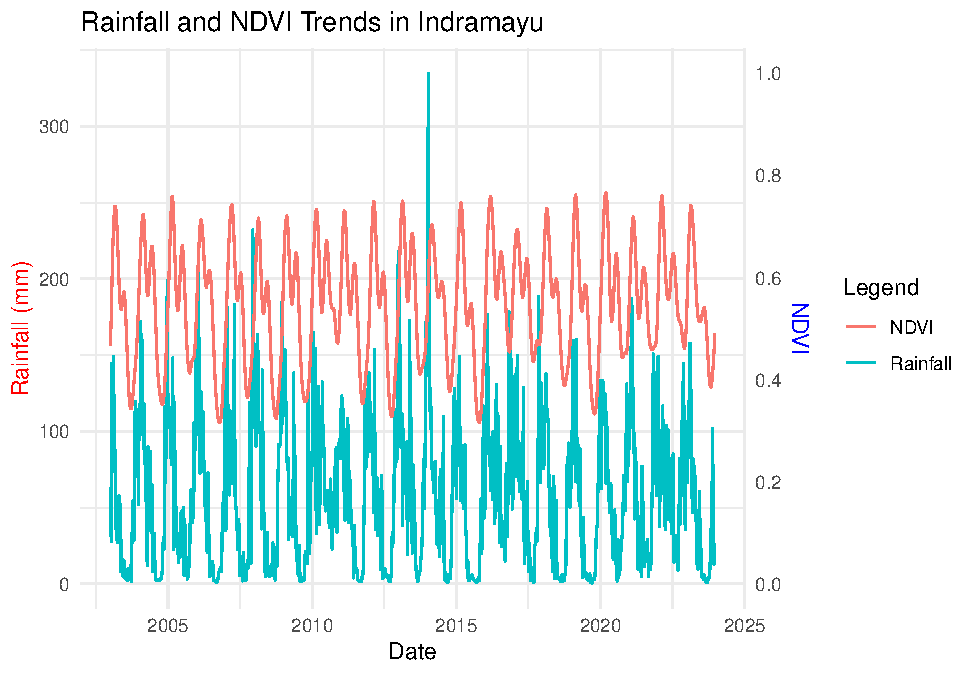
\includegraphics{BI_VegetationResponse_Project_HarvardX_Ph125_9x_files/figure-latex/eda_rain_ndvi_trend-1} \end{center}

\begin{Shaded}
\begin{Highlighting}[]
\CommentTok{\# Track and print processing time}
\NormalTok{end\_time }\OtherTok{\textless{}{-}} \FunctionTok{Sys.time}\NormalTok{()}
\NormalTok{processing\_time }\OtherTok{\textless{}{-}}\NormalTok{ end\_time }\SpecialCharTok{{-}}\NormalTok{ start\_time}
\FunctionTok{print}\NormalTok{(}\FunctionTok{paste}\NormalTok{(}\StringTok{"Processing time: "}\NormalTok{, processing\_time))}
\end{Highlighting}
\end{Shaded}

\begin{verbatim}
## [1] "Processing time:  7.52352499961853"
\end{verbatim}

This code will generate a time-series plot showing rainfall and NDVI
trends for Indramayu. You should see how NDVI changes in response to
rainfall, with potential seasonal variations.

\subsection{Correlation Analysis}\label{correlation-analysis}

To understand the relationship between rainfall and NDVI, we perform a
correlation analysis, particularly focusing on \textbf{lagged
correlations}, where rainfall from earlier periods may affect NDVI in
later periods.

\begin{Shaded}
\begin{Highlighting}[]
\CommentTok{\# Load necessary libraries and track time}
\NormalTok{start\_time }\OtherTok{\textless{}{-}} \FunctionTok{Sys.time}\NormalTok{()}

\CommentTok{\# Create lagged rainfall features (1 to 6 dekads before)}
\NormalTok{indramayu\_rainfall }\OtherTok{\textless{}{-}}\NormalTok{ indramayu\_rainfall }\SpecialCharTok{\%\textgreater{}\%}
\NormalTok{  dplyr}\SpecialCharTok{::}\FunctionTok{arrange}\NormalTok{(date) }\SpecialCharTok{\%\textgreater{}\%}
\NormalTok{  dplyr}\SpecialCharTok{::}\FunctionTok{mutate}\NormalTok{(}\AttributeTok{rainfall\_lag\_1 =}\NormalTok{ dplyr}\SpecialCharTok{::}\FunctionTok{lag}\NormalTok{(rfh, }\DecValTok{1}\NormalTok{),}
                \AttributeTok{rainfall\_lag\_2 =}\NormalTok{ dplyr}\SpecialCharTok{::}\FunctionTok{lag}\NormalTok{(rfh, }\DecValTok{2}\NormalTok{),}
                \AttributeTok{rainfall\_lag\_3 =}\NormalTok{ dplyr}\SpecialCharTok{::}\FunctionTok{lag}\NormalTok{(rfh, }\DecValTok{3}\NormalTok{),}
                \AttributeTok{rainfall\_lag\_4 =}\NormalTok{ dplyr}\SpecialCharTok{::}\FunctionTok{lag}\NormalTok{(rfh, }\DecValTok{4}\NormalTok{),}
                \AttributeTok{rainfall\_lag\_5 =}\NormalTok{ dplyr}\SpecialCharTok{::}\FunctionTok{lag}\NormalTok{(rfh, }\DecValTok{5}\NormalTok{),}
                \AttributeTok{rainfall\_lag\_6 =}\NormalTok{ dplyr}\SpecialCharTok{::}\FunctionTok{lag}\NormalTok{(rfh, }\DecValTok{6}\NormalTok{))}

\CommentTok{\# Merge rainfall and NDVI datasets by date}
\NormalTok{merged\_data }\OtherTok{\textless{}{-}}\NormalTok{ dplyr}\SpecialCharTok{::}\FunctionTok{inner\_join}\NormalTok{(indramayu\_ndvi, }
\NormalTok{                                 indramayu\_rainfall, }
                                 \AttributeTok{by =} \StringTok{"date"}\NormalTok{)}

\CommentTok{\# Calculate correlation between NDVI and lagged rainfall features}
\NormalTok{cor\_lag\_1 }\OtherTok{\textless{}{-}}\NormalTok{ stats}\SpecialCharTok{::}\FunctionTok{cor}\NormalTok{(merged\_data}\SpecialCharTok{$}\NormalTok{vim, }
\NormalTok{                        merged\_data}\SpecialCharTok{$}\NormalTok{rainfall\_lag\_1, }
                        \AttributeTok{use =} \StringTok{"complete.obs"}\NormalTok{)}
\NormalTok{cor\_lag\_2 }\OtherTok{\textless{}{-}}\NormalTok{ stats}\SpecialCharTok{::}\FunctionTok{cor}\NormalTok{(merged\_data}\SpecialCharTok{$}\NormalTok{vim, }
\NormalTok{                        merged\_data}\SpecialCharTok{$}\NormalTok{rainfall\_lag\_2, }
                        \AttributeTok{use =} \StringTok{"complete.obs"}\NormalTok{)}
\NormalTok{cor\_lag\_3 }\OtherTok{\textless{}{-}}\NormalTok{ stats}\SpecialCharTok{::}\FunctionTok{cor}\NormalTok{(merged\_data}\SpecialCharTok{$}\NormalTok{vim, }
\NormalTok{                        merged\_data}\SpecialCharTok{$}\NormalTok{rainfall\_lag\_3, }
                        \AttributeTok{use =} \StringTok{"complete.obs"}\NormalTok{)}
\NormalTok{cor\_lag\_4 }\OtherTok{\textless{}{-}}\NormalTok{ stats}\SpecialCharTok{::}\FunctionTok{cor}\NormalTok{(merged\_data}\SpecialCharTok{$}\NormalTok{vim, }
\NormalTok{                        merged\_data}\SpecialCharTok{$}\NormalTok{rainfall\_lag\_4, }
                        \AttributeTok{use =} \StringTok{"complete.obs"}\NormalTok{)}
\NormalTok{cor\_lag\_5 }\OtherTok{\textless{}{-}}\NormalTok{ stats}\SpecialCharTok{::}\FunctionTok{cor}\NormalTok{(merged\_data}\SpecialCharTok{$}\NormalTok{vim, }
\NormalTok{                        merged\_data}\SpecialCharTok{$}\NormalTok{rainfall\_lag\_5, }
                        \AttributeTok{use =} \StringTok{"complete.obs"}\NormalTok{)}
\NormalTok{cor\_lag\_6 }\OtherTok{\textless{}{-}}\NormalTok{ stats}\SpecialCharTok{::}\FunctionTok{cor}\NormalTok{(merged\_data}\SpecialCharTok{$}\NormalTok{vim, }
\NormalTok{                        merged\_data}\SpecialCharTok{$}\NormalTok{rainfall\_lag\_6, }
                        \AttributeTok{use =} \StringTok{"complete.obs"}\NormalTok{)}

\CommentTok{\# Print correlation results}
\NormalTok{base}\SpecialCharTok{::}\FunctionTok{print}\NormalTok{(base}\SpecialCharTok{::}\FunctionTok{paste}\NormalTok{(}\StringTok{"Correlation between NDVI and Rainfall Lag 1: "}\NormalTok{, }
\NormalTok{                        base}\SpecialCharTok{::}\FunctionTok{round}\NormalTok{(cor\_lag\_1, }\DecValTok{3}\NormalTok{)))}
\end{Highlighting}
\end{Shaded}

\begin{verbatim}
## [1] "Correlation between NDVI and Rainfall Lag 1:  0.495"
\end{verbatim}

\begin{Shaded}
\begin{Highlighting}[]
\NormalTok{base}\SpecialCharTok{::}\FunctionTok{print}\NormalTok{(base}\SpecialCharTok{::}\FunctionTok{paste}\NormalTok{(}\StringTok{"Correlation between NDVI and Rainfall Lag 2: "}\NormalTok{, }
\NormalTok{                        base}\SpecialCharTok{::}\FunctionTok{round}\NormalTok{(cor\_lag\_2, }\DecValTok{3}\NormalTok{)))}
\end{Highlighting}
\end{Shaded}

\begin{verbatim}
## [1] "Correlation between NDVI and Rainfall Lag 2:  0.581"
\end{verbatim}

\begin{Shaded}
\begin{Highlighting}[]
\NormalTok{base}\SpecialCharTok{::}\FunctionTok{print}\NormalTok{(base}\SpecialCharTok{::}\FunctionTok{paste}\NormalTok{(}\StringTok{"Correlation between NDVI and Rainfall Lag 3: "}\NormalTok{, }
\NormalTok{                        base}\SpecialCharTok{::}\FunctionTok{round}\NormalTok{(cor\_lag\_3, }\DecValTok{3}\NormalTok{)))}
\end{Highlighting}
\end{Shaded}

\begin{verbatim}
## [1] "Correlation between NDVI and Rainfall Lag 3:  0.644"
\end{verbatim}

\begin{Shaded}
\begin{Highlighting}[]
\NormalTok{base}\SpecialCharTok{::}\FunctionTok{print}\NormalTok{(base}\SpecialCharTok{::}\FunctionTok{paste}\NormalTok{(}\StringTok{"Correlation between NDVI and Rainfall Lag 4: "}\NormalTok{, }
\NormalTok{                        base}\SpecialCharTok{::}\FunctionTok{round}\NormalTok{(cor\_lag\_4, }\DecValTok{3}\NormalTok{)))}
\end{Highlighting}
\end{Shaded}

\begin{verbatim}
## [1] "Correlation between NDVI and Rainfall Lag 4:  0.684"
\end{verbatim}

\begin{Shaded}
\begin{Highlighting}[]
\NormalTok{base}\SpecialCharTok{::}\FunctionTok{print}\NormalTok{(base}\SpecialCharTok{::}\FunctionTok{paste}\NormalTok{(}\StringTok{"Correlation between NDVI and Rainfall Lag 5: "}\NormalTok{, }
\NormalTok{                        base}\SpecialCharTok{::}\FunctionTok{round}\NormalTok{(cor\_lag\_5, }\DecValTok{3}\NormalTok{)))}
\end{Highlighting}
\end{Shaded}

\begin{verbatim}
## [1] "Correlation between NDVI and Rainfall Lag 5:  0.699"
\end{verbatim}

\begin{Shaded}
\begin{Highlighting}[]
\NormalTok{base}\SpecialCharTok{::}\FunctionTok{print}\NormalTok{(base}\SpecialCharTok{::}\FunctionTok{paste}\NormalTok{(}\StringTok{"Correlation between NDVI and Rainfall Lag 6: "}\NormalTok{, }
\NormalTok{                        base}\SpecialCharTok{::}\FunctionTok{round}\NormalTok{(cor\_lag\_6, }\DecValTok{3}\NormalTok{)))}
\end{Highlighting}
\end{Shaded}

\begin{verbatim}
## [1] "Correlation between NDVI and Rainfall Lag 6:  0.689"
\end{verbatim}

\begin{Shaded}
\begin{Highlighting}[]
\CommentTok{\# Track and print processing time}
\NormalTok{end\_time }\OtherTok{\textless{}{-}} \FunctionTok{Sys.time}\NormalTok{()}
\NormalTok{processing\_time }\OtherTok{\textless{}{-}}\NormalTok{ end\_time }\SpecialCharTok{{-}}\NormalTok{ start\_time}
\FunctionTok{print}\NormalTok{(}\FunctionTok{paste}\NormalTok{(}\StringTok{"Processing time: "}\NormalTok{, processing\_time))}
\end{Highlighting}
\end{Shaded}

\begin{verbatim}
## [1] "Processing time:  0.0308229923248291"
\end{verbatim}

This script calculates and prints the correlations between NDVI and
lagged rainfall at 1, 2, and 3 dekads before. These correlations can
help identify the time-lagged relationship between rainfall and
vegetation health.

\subsection{Rainfall and NDVI
Anomalies}\label{rainfall-and-ndvi-anomalies}

Understanding anomalies is crucial for detecting unusual events in the
rainfall and NDVI data, which could indicate extreme weather or
vegetation stress. In this section, we plot anomalies for both
variables.

\begin{Shaded}
\begin{Highlighting}[]
\CommentTok{\# Load necessary libraries and track time}
\NormalTok{start\_time }\OtherTok{\textless{}{-}} \FunctionTok{Sys.time}\NormalTok{()}

\CommentTok{\# Filter anomalies from both datasets and convert to numeric}
\NormalTok{indramayu\_rainfall\_anomalies }\OtherTok{\textless{}{-}}\NormalTok{ indramayu\_rainfall }\SpecialCharTok{\%\textgreater{}\%}
\NormalTok{  dplyr}\SpecialCharTok{::}\FunctionTok{select}\NormalTok{(date, rfq) }\SpecialCharTok{\%\textgreater{}\%}
\NormalTok{  dplyr}\SpecialCharTok{::}\FunctionTok{rename}\NormalTok{(}\AttributeTok{rainfall\_anomaly =}\NormalTok{ rfq) }\SpecialCharTok{\%\textgreater{}\%}
\NormalTok{  dplyr}\SpecialCharTok{::}\FunctionTok{mutate}\NormalTok{(}\AttributeTok{rainfall\_anomaly =} \FunctionTok{as.numeric}\NormalTok{(rainfall\_anomaly))}

\NormalTok{indramayu\_ndvi\_anomalies }\OtherTok{\textless{}{-}}\NormalTok{ indramayu\_ndvi }\SpecialCharTok{\%\textgreater{}\%}
\NormalTok{  dplyr}\SpecialCharTok{::}\FunctionTok{select}\NormalTok{(date, viq) }\SpecialCharTok{\%\textgreater{}\%}
\NormalTok{  dplyr}\SpecialCharTok{::}\FunctionTok{rename}\NormalTok{(}\AttributeTok{ndvi\_anomaly =}\NormalTok{ viq) }\SpecialCharTok{\%\textgreater{}\%}
\NormalTok{  dplyr}\SpecialCharTok{::}\FunctionTok{mutate}\NormalTok{(}\AttributeTok{ndvi\_anomaly =} \FunctionTok{as.numeric}\NormalTok{(ndvi\_anomaly))}

\CommentTok{\# Merge anomaly data by date}
\NormalTok{anomalies\_data }\OtherTok{\textless{}{-}}\NormalTok{ dplyr}\SpecialCharTok{::}\FunctionTok{inner\_join}\NormalTok{(indramayu\_rainfall\_anomalies, }
\NormalTok{                                    indramayu\_ndvi\_anomalies, }
                                    \AttributeTok{by =} \StringTok{"date"}\NormalTok{)}

\CommentTok{\# Plot anomalies on a single Y{-}axis ranging from 0 to 200\%}
\NormalTok{ggplot2}\SpecialCharTok{::}\FunctionTok{ggplot}\NormalTok{(anomalies\_data, ggplot2}\SpecialCharTok{::}\FunctionTok{aes}\NormalTok{(}\AttributeTok{x =}\NormalTok{ date)) }\SpecialCharTok{+}
\NormalTok{  ggplot2}\SpecialCharTok{::}\FunctionTok{geom\_line}\NormalTok{(ggplot2}\SpecialCharTok{::}\FunctionTok{aes}\NormalTok{(}\AttributeTok{y =}\NormalTok{ rainfall\_anomaly, }
                                  \AttributeTok{color =} \StringTok{"Rainfall Anomaly"}\NormalTok{)) }\SpecialCharTok{+}
\NormalTok{  ggplot2}\SpecialCharTok{::}\FunctionTok{geom\_line}\NormalTok{(ggplot2}\SpecialCharTok{::}\FunctionTok{aes}\NormalTok{(}\AttributeTok{y =}\NormalTok{ ndvi\_anomaly, }
                                  \AttributeTok{color =} \StringTok{"NDVI Anomaly"}\NormalTok{)) }\SpecialCharTok{+}
\NormalTok{  ggplot2}\SpecialCharTok{::}\FunctionTok{scale\_y\_continuous}\NormalTok{(}\AttributeTok{limits =} \FunctionTok{c}\NormalTok{(}\DecValTok{0}\NormalTok{, }\DecValTok{200}\NormalTok{), }
                              \AttributeTok{breaks =} \FunctionTok{seq}\NormalTok{(}\DecValTok{0}\NormalTok{, }\DecValTok{200}\NormalTok{, }\DecValTok{20}\NormalTok{)) }\SpecialCharTok{+}
\NormalTok{  ggplot2}\SpecialCharTok{::}\FunctionTok{labs}\NormalTok{(}\AttributeTok{title =} \StringTok{"Rainfall and NDVI Anomalies in Indramayu"}\NormalTok{,}
       \AttributeTok{x =} \StringTok{"Date"}\NormalTok{, }
       \AttributeTok{y =} \StringTok{"Anomaly (\%)"}\NormalTok{,}
       \AttributeTok{color =} \StringTok{"Legend"}\NormalTok{) }\SpecialCharTok{+}
\NormalTok{  ggplot2}\SpecialCharTok{::}\FunctionTok{theme\_minimal}\NormalTok{()}
\end{Highlighting}
\end{Shaded}

\begin{center}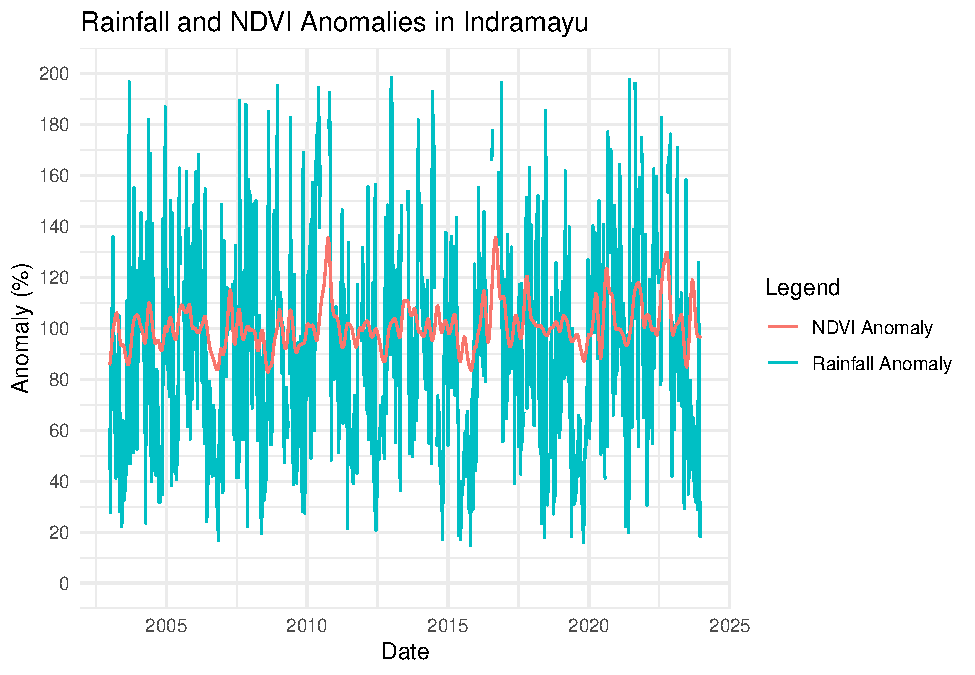
\includegraphics{BI_VegetationResponse_Project_HarvardX_Ph125_9x_files/figure-latex/eda_rain_ndvi_anom-1} \end{center}

\begin{Shaded}
\begin{Highlighting}[]
\CommentTok{\# Track and print processing time}
\NormalTok{end\_time }\OtherTok{\textless{}{-}} \FunctionTok{Sys.time}\NormalTok{()}
\NormalTok{processing\_time }\OtherTok{\textless{}{-}}\NormalTok{ end\_time }\SpecialCharTok{{-}}\NormalTok{ start\_time}
\FunctionTok{print}\NormalTok{(}\FunctionTok{paste}\NormalTok{(}\StringTok{"Processing time: "}\NormalTok{, processing\_time))}
\end{Highlighting}
\end{Shaded}

\begin{verbatim}
## [1] "Processing time:  0.353729963302612"
\end{verbatim}

This script will visualize the anomalies for both rainfall and NDVI,
helping to detect any deviations from average patterns over time.

\begin{center}\rule{0.5\linewidth}{0.5pt}\end{center}

\section{Methods and Machine Learning
Models}\label{methods-and-machine-learning-models}

\subsection{Problem Framing}\label{problem-framing}

The goal of this project is to predict \textbf{NDVI} (Normalized
Difference Vegetation Index), a key indicator of vegetation health,
using \textbf{rainfall data} as the primary predictor. This predictive
problem is framed as a \textbf{supervised learning task} where we aim to
model the time-lagged effects of rainfall on NDVI. Given the structure
of the data (where vegetation response to rainfall is delayed), this
problem also incorporates temporal elements through the use of
\textbf{lagged features}.

Supervised Learning Setup:

\begin{itemize}
\tightlist
\item
  \textbf{Input}: Rainfall data (including lagged rainfall values)
\item
  \textbf{Output}: NDVI values (target variable)
\item
  \textbf{Type of task}: Regression, where the goal is to predict
  continuous NDVI values.
\end{itemize}

To model this relationship, we will explore several approaches:

\begin{itemize}
\tightlist
\item
  \textbf{Time-lagged linear regression}: A simple, interpretable model
  to understand how lagged rainfall affects NDVI.
\item
  \textbf{Random Forest regression}: A more flexible, non-linear model
  to capture complex interactions.
\item
  \textbf{Time-series forecasting models} (optional): For exploring
  future NDVI predictions based on past data.
\end{itemize}

\subsection{Time-Lagged Regression
Model}\label{time-lagged-regression-model}

Linear regression is a common approach for modeling the relationship
between a dependent variable \(y\) (in this case, NDVI) and one or more
independent variables \(X\) (lagged rainfall values). The general form
of a \textbf{multiple linear regression} model is:

\[
y_t = \beta_0 + \beta_1 X_{t-1} + \beta_2 X_{t-2} + ... + \beta_n X_{t-n} + \epsilon
\]

Where: - \(y_t\) is the NDVI value at time \(t\). -
\(X_{t-1}, X_{t-2}, ..., X_{t-n}\) are the lagged rainfall values from
previous periods (dekads). - \(\beta_0\) is the intercept. -
\(\beta_1, \beta_2, ..., \beta_n\) are the coefficients representing the
effect of rainfall at different lags. - \(\epsilon\) is the error term.

In our case, we use up to \textbf{6 lagged rainfall values} to capture
the delayed effect of rainfall on vegetation health. This approach
allows us to quantify how rainfall from previous periods affects NDVI,
offering insights into both short-term and long-term vegetation
responses.

\begin{Shaded}
\begin{Highlighting}[]
\CommentTok{\# Load necessary libraries and track time}
\NormalTok{start\_time }\OtherTok{\textless{}{-}} \FunctionTok{Sys.time}\NormalTok{()}

\CommentTok{\# Create lagged rainfall features (1 to 6 dekads before)}
\NormalTok{indramayu\_rainfall }\OtherTok{\textless{}{-}}\NormalTok{ indramayu\_rainfall }\SpecialCharTok{\%\textgreater{}\%}
\NormalTok{  dplyr}\SpecialCharTok{::}\FunctionTok{arrange}\NormalTok{(date) }\SpecialCharTok{\%\textgreater{}\%}
\NormalTok{  dplyr}\SpecialCharTok{::}\FunctionTok{mutate}\NormalTok{(}\AttributeTok{rainfall\_lag\_1 =}\NormalTok{ dplyr}\SpecialCharTok{::}\FunctionTok{lag}\NormalTok{(rfh, }\DecValTok{1}\NormalTok{),}
                \AttributeTok{rainfall\_lag\_2 =}\NormalTok{ dplyr}\SpecialCharTok{::}\FunctionTok{lag}\NormalTok{(rfh, }\DecValTok{2}\NormalTok{),}
                \AttributeTok{rainfall\_lag\_3 =}\NormalTok{ dplyr}\SpecialCharTok{::}\FunctionTok{lag}\NormalTok{(rfh, }\DecValTok{3}\NormalTok{),}
                \AttributeTok{rainfall\_lag\_4 =}\NormalTok{ dplyr}\SpecialCharTok{::}\FunctionTok{lag}\NormalTok{(rfh, }\DecValTok{4}\NormalTok{),}
                \AttributeTok{rainfall\_lag\_5 =}\NormalTok{ dplyr}\SpecialCharTok{::}\FunctionTok{lag}\NormalTok{(rfh, }\DecValTok{5}\NormalTok{),}
                \AttributeTok{rainfall\_lag\_6 =}\NormalTok{ dplyr}\SpecialCharTok{::}\FunctionTok{lag}\NormalTok{(rfh, }\DecValTok{6}\NormalTok{))}

\CommentTok{\# Merge rainfall and NDVI datasets by date}
\NormalTok{merged\_data }\OtherTok{\textless{}{-}}\NormalTok{ dplyr}\SpecialCharTok{::}\FunctionTok{inner\_join}\NormalTok{(indramayu\_ndvi, }
\NormalTok{                                 indramayu\_rainfall, }
                                 \AttributeTok{by =} \StringTok{"date"}\NormalTok{)}

\CommentTok{\# Build linear regression model with lagged rainfall features}
\NormalTok{linear\_model }\OtherTok{\textless{}{-}}\NormalTok{ stats}\SpecialCharTok{::}\FunctionTok{lm}\NormalTok{(vim }\SpecialCharTok{\textasciitilde{}}\NormalTok{ rainfall\_lag\_1 }\SpecialCharTok{+}\NormalTok{ rainfall\_lag\_2 }\SpecialCharTok{+} 
\NormalTok{                          rainfall\_lag\_3 }\SpecialCharTok{+}\NormalTok{ rainfall\_lag\_4 }\SpecialCharTok{+}\NormalTok{ rainfall\_lag\_5 }
                          \SpecialCharTok{+}\NormalTok{ rainfall\_lag\_6, }\AttributeTok{data =}\NormalTok{ merged\_data)}

\CommentTok{\# Print model summary}
\NormalTok{base}\SpecialCharTok{::}\FunctionTok{summary}\NormalTok{(linear\_model)}
\end{Highlighting}
\end{Shaded}

\begin{verbatim}
## 
## Call:
## stats::lm(formula = vim ~ rainfall_lag_1 + rainfall_lag_2 + rainfall_lag_3 + 
##     rainfall_lag_4 + rainfall_lag_5 + rainfall_lag_6, data = merged_data)
## 
## Residuals:
##       Min        1Q    Median        3Q       Max 
## -0.172800 -0.049174 -0.007631  0.048168  0.183816 
## 
## Coefficients:
##                 Estimate Std. Error t value Pr(>|t|)    
## (Intercept)    4.152e-01  4.360e-03  95.234  < 2e-16 ***
## rainfall_lag_1 8.595e-05  6.919e-05   1.242  0.21454    
## rainfall_lag_2 2.477e-04  7.643e-05   3.241  0.00125 ** 
## rainfall_lag_3 3.235e-04  7.739e-05   4.180 3.27e-05 ***
## rainfall_lag_4 4.495e-04  7.745e-05   5.804 9.60e-09 ***
## rainfall_lag_5 5.125e-04  7.618e-05   6.728 3.44e-11 ***
## rainfall_lag_6 6.899e-04  6.894e-05  10.007  < 2e-16 ***
## ---
## Signif. codes:  0 '***' 0.001 '**' 0.01 '*' 0.05 '.' 0.1 ' ' 1
## 
## Residual standard error: 0.06623 on 743 degrees of freedom
##   (6 observations deleted due to missingness)
## Multiple R-squared:  0.6627, Adjusted R-squared:   0.66 
## F-statistic: 243.3 on 6 and 743 DF,  p-value: < 2.2e-16
\end{verbatim}

\begin{Shaded}
\begin{Highlighting}[]
\CommentTok{\# Track and print processing time}
\NormalTok{end\_time }\OtherTok{\textless{}{-}} \FunctionTok{Sys.time}\NormalTok{()}
\NormalTok{processing\_time }\OtherTok{\textless{}{-}}\NormalTok{ end\_time }\SpecialCharTok{{-}}\NormalTok{ start\_time}
\FunctionTok{print}\NormalTok{(}\FunctionTok{paste}\NormalTok{(}\StringTok{"Processing time: "}\NormalTok{, processing\_time))}
\end{Highlighting}
\end{Shaded}

\begin{verbatim}
## [1] "Processing time:  0.119018077850342"
\end{verbatim}

\textbf{Interpretation:}

\begin{itemize}
\tightlist
\item
  The coefficients for the lagged rainfall variables will tell us how
  much each lagged period (dekad) contributes to NDVI changes.
\item
  We can assess the \textbf{p-values} to determine which lags are
  statistically significant predictors of NDVI.
\end{itemize}

\subsection{Random Forest Regression}\label{random-forest-regression}

\textbf{Random Forest} is a non-linear, ensemble learning method that
builds multiple decision trees and averages their predictions to reduce
overfitting and improve generalization. Random Forest can handle complex
interactions between features, making it a good choice for modeling the
\textbf{non-linear} relationships between rainfall and NDVI.
Additionally, it can naturally incorporate \textbf{feature importance
analysis}, helping us identify which lagged rainfall values have the
most influence on NDVI.

The basic idea of Random Forest regression can be described as:

\[
\hat{y} = \frac{1}{T} \sum_{t=1}^{T} f_t(X)
\]

Where: - \(\hat{y}\) is the predicted NDVI value. - \(T\) is the number
of decision trees. - \(f_t(X)\) is the prediction from the \(t\)-th
decision tree based on the input features \(X\) (lagged rainfall
values).

\begin{Shaded}
\begin{Highlighting}[]
\CommentTok{\# Load necessary libraries and track time}
\NormalTok{start\_time }\OtherTok{\textless{}{-}} \FunctionTok{Sys.time}\NormalTok{()}

\CommentTok{\# Create lagged rainfall features (as done earlier)}
\NormalTok{indramayu\_rainfall }\OtherTok{\textless{}{-}}\NormalTok{ indramayu\_rainfall }\SpecialCharTok{\%\textgreater{}\%}
\NormalTok{  dplyr}\SpecialCharTok{::}\FunctionTok{arrange}\NormalTok{(date) }\SpecialCharTok{\%\textgreater{}\%}
\NormalTok{  dplyr}\SpecialCharTok{::}\FunctionTok{mutate}\NormalTok{(}\AttributeTok{rainfall\_lag\_1 =}\NormalTok{ dplyr}\SpecialCharTok{::}\FunctionTok{lag}\NormalTok{(rfh, }\DecValTok{1}\NormalTok{),}
                \AttributeTok{rainfall\_lag\_2 =}\NormalTok{ dplyr}\SpecialCharTok{::}\FunctionTok{lag}\NormalTok{(rfh, }\DecValTok{2}\NormalTok{),}
                \AttributeTok{rainfall\_lag\_3 =}\NormalTok{ dplyr}\SpecialCharTok{::}\FunctionTok{lag}\NormalTok{(rfh, }\DecValTok{3}\NormalTok{),}
                \AttributeTok{rainfall\_lag\_4 =}\NormalTok{ dplyr}\SpecialCharTok{::}\FunctionTok{lag}\NormalTok{(rfh, }\DecValTok{4}\NormalTok{),}
                \AttributeTok{rainfall\_lag\_5 =}\NormalTok{ dplyr}\SpecialCharTok{::}\FunctionTok{lag}\NormalTok{(rfh, }\DecValTok{5}\NormalTok{),}
                \AttributeTok{rainfall\_lag\_6 =}\NormalTok{ dplyr}\SpecialCharTok{::}\FunctionTok{lag}\NormalTok{(rfh, }\DecValTok{6}\NormalTok{))}

\CommentTok{\# Merge rainfall and NDVI datasets by date}
\NormalTok{merged\_data }\OtherTok{\textless{}{-}}\NormalTok{ dplyr}\SpecialCharTok{::}\FunctionTok{inner\_join}\NormalTok{(indramayu\_ndvi, }
\NormalTok{                                 indramayu\_rainfall, }
                                 \AttributeTok{by =} \StringTok{"date"}\NormalTok{)}

\CommentTok{\# Remove rows with missing values (NA) from the merged dataset}
\NormalTok{cleaned\_data }\OtherTok{\textless{}{-}} \FunctionTok{na.omit}\NormalTok{(merged\_data)}

\CommentTok{\# Build Random Forest regression model}
\NormalTok{rf\_model }\OtherTok{\textless{}{-}}\NormalTok{ randomForest}\SpecialCharTok{::}\FunctionTok{randomForest}\NormalTok{(vim }\SpecialCharTok{\textasciitilde{}}\NormalTok{ rainfall\_lag\_1 }\SpecialCharTok{+}\NormalTok{ rainfall\_lag\_2 }\SpecialCharTok{+} 
\NormalTok{                                       rainfall\_lag\_3 }\SpecialCharTok{+}\NormalTok{ rainfall\_lag\_4 }\SpecialCharTok{+} 
\NormalTok{                                       rainfall\_lag\_5 }\SpecialCharTok{+}\NormalTok{ rainfall\_lag\_6, }
                                       \AttributeTok{data =}\NormalTok{ cleaned\_data, }
                                       \AttributeTok{ntree =} \DecValTok{500}\NormalTok{, }
                                       \AttributeTok{importance =} \ConstantTok{TRUE}\NormalTok{)}

\CommentTok{\# Print Random Forest model summary}
\NormalTok{base}\SpecialCharTok{::}\FunctionTok{print}\NormalTok{(rf\_model)}
\end{Highlighting}
\end{Shaded}

\begin{verbatim}
## 
## Call:
##  randomForest(formula = vim ~ rainfall_lag_1 + rainfall_lag_2 +      rainfall_lag_3 + rainfall_lag_4 + rainfall_lag_5 + rainfall_lag_6,      data = cleaned_data, ntree = 500, importance = TRUE) 
##                Type of random forest: regression
##                      Number of trees: 500
## No. of variables tried at each split: 2
## 
##           Mean of squared residuals: 0.003348155
##                     % Var explained: 74.01
\end{verbatim}

\begin{Shaded}
\begin{Highlighting}[]
\CommentTok{\# Plot feature importance}
\NormalTok{randomForest}\SpecialCharTok{::}\FunctionTok{importance}\NormalTok{(rf\_model)}
\end{Highlighting}
\end{Shaded}

\begin{verbatim}
##                 %IncMSE IncNodePurity
## rainfall_lag_1 18.26808     0.5372938
## rainfall_lag_2 17.10857     0.8880499
## rainfall_lag_3 21.22461     1.2655402
## rainfall_lag_4 27.30987     1.8626793
## rainfall_lag_5 35.52283     2.4676570
## rainfall_lag_6 44.46729     2.4102751
\end{verbatim}

\begin{Shaded}
\begin{Highlighting}[]
\NormalTok{randomForest}\SpecialCharTok{::}\FunctionTok{varImpPlot}\NormalTok{(rf\_model)}
\end{Highlighting}
\end{Shaded}

\begin{center}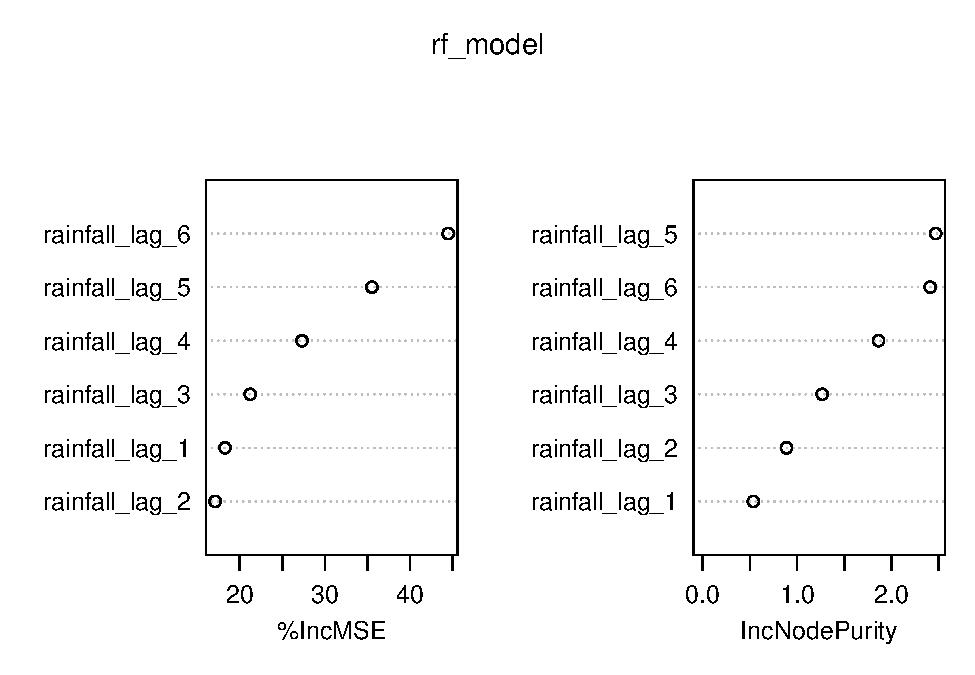
\includegraphics{BI_VegetationResponse_Project_HarvardX_Ph125_9x_files/figure-latex/ml_rain_ndvi_randomforest-1} \end{center}

\begin{Shaded}
\begin{Highlighting}[]
\CommentTok{\# Track and print processing time}
\NormalTok{end\_time }\OtherTok{\textless{}{-}} \FunctionTok{Sys.time}\NormalTok{()}
\NormalTok{processing\_time }\OtherTok{\textless{}{-}}\NormalTok{ end\_time }\SpecialCharTok{{-}}\NormalTok{ start\_time}
\FunctionTok{print}\NormalTok{(}\FunctionTok{paste}\NormalTok{(}\StringTok{"Processing time: "}\NormalTok{, processing\_time))}
\end{Highlighting}
\end{Shaded}

\begin{verbatim}
## [1] "Processing time:  1.50602889060974"
\end{verbatim}

\textbf{Interpretation:}

\begin{itemize}
\tightlist
\item
  The \textbf{importance plot} shows which lagged rainfall features
  contribute the most to predicting NDVI.
\item
  \textbf{Random Forest} can capture \textbf{non-linear relationships}
  between rainfall and NDVI, which may not be apparent in a linear
  regression model.
\end{itemize}

\subsection{Time-Series Regression Model with External Predictors
(ARIMAX)}\label{time-series-regression-model-with-external-predictors-arimax}

In addition to \textbf{Linear Regression} and \textbf{Random Forest}, we
will incorporate an \textbf{ARIMAX} model to predict NDVI based on both
past NDVI values and rainfall as an external predictor. The
\textbf{ARIMAX} model is an extension of ARIMA, specifically designed
for time-series forecasting with exogenous inputs (e.g., rainfall).

ARIMAX is defined by three main parameters (\(p\), \(d\), \(q\)),
similar to ARIMA, but it also incorporates external regressors:

\begin{itemize}
\tightlist
\item
  \(p\): The number of autoregressive terms.
\item
  \(d\): The degree of differencing to make the time series stationary.
\item
  \(q\): The number of moving average terms.
\item
  \(x_{reg}\): External regressors (in this case, rainfall).
\end{itemize}

By fitting an \textbf{ARIMAX} model to the \textbf{NDVI} time series
with \textbf{rainfall} as the exogenous variable, we can predict NDVI
based on both the historical values of NDVI and rainfall data, offering
a model that incorporates both \textbf{time-series} and
\textbf{regression} components.

The ARIMAX model can be written as:

\[
NDVI_t = \phi_0 + \sum_{i=1}^{p} \phi_i NDVI_{t-i} + \sum_{j=1}^{q} \theta_j \epsilon_{t-j} + \sum_{k=1}^{m} \beta_k Rainfall_{t-k} + \epsilon_t
\]

Where: - \(NDVI_t\) is the NDVI at time \(t\). - \(\phi_0\) is the
intercept term. - \(\phi_i\) are the autoregressive coefficients (based
on previous NDVI values). - \(\theta_j\) are the moving average
coefficients. - \(\beta_k\) are the coefficients for the external
regressors (rainfall at time \(t-k\)). - \(\epsilon_t\) is the white
noise error term.

\textbf{Advantages and Limitations:}

\begin{itemize}
\tightlist
\item
  \textbf{Advantages}: ARIMAX combines both time-series analysis and
  regression, allowing for the inclusion of external predictors
  (rainfall) in the NDVI prediction.
\item
  \textbf{Limitations}: ARIMAX assumes linear relationships and may
  struggle with capturing non-linear dynamics, for which models like
  \textbf{Random Forest} may perform better.
\end{itemize}

\begin{Shaded}
\begin{Highlighting}[]
\CommentTok{\# Load necessary libraries and track time}
\NormalTok{start\_time }\OtherTok{\textless{}{-}} \FunctionTok{Sys.time}\NormalTok{()}

\CommentTok{\# Prepare NDVI data as a time series and rainfall as the exogenous variable}
\CommentTok{\# Assuming dekadal data (36 periods per year)}
\NormalTok{ndvi\_ts }\OtherTok{\textless{}{-}}\NormalTok{ stats}\SpecialCharTok{::}\FunctionTok{ts}\NormalTok{(merged\_data}\SpecialCharTok{$}\NormalTok{vim, }\AttributeTok{frequency =} \DecValTok{36}\NormalTok{)  }
\NormalTok{rainfall\_exog }\OtherTok{\textless{}{-}}\NormalTok{ merged\_data}\SpecialCharTok{$}\NormalTok{rfh  }\CommentTok{\# Use rainfall as the external regressor}

\CommentTok{\# Fit ARIMAX model using auto.arima with external regressors (rainfall)}
\NormalTok{arimax\_model }\OtherTok{\textless{}{-}}\NormalTok{ forecast}\SpecialCharTok{::}\FunctionTok{auto.arima}\NormalTok{(ndvi\_ts, }\AttributeTok{xreg =}\NormalTok{ rainfall\_exog)}

\CommentTok{\# Print ARIMAX model summary}
\NormalTok{base}\SpecialCharTok{::}\FunctionTok{summary}\NormalTok{(arimax\_model)}
\end{Highlighting}
\end{Shaded}

\begin{verbatim}
## Series: ndvi_ts 
## Regression with ARIMA(0,0,0)(1,1,0)[36] errors 
## 
## Coefficients:
##          sar1  drift   xreg
##       -0.4586  0e+00  5e-04
## s.e.   0.0333  1e-04  1e-04
## 
## sigma^2 = 0.002804:  log likelihood = 1091.29
## AIC=-2174.57   AICc=-2174.52   BIC=-2156.26
## 
## Training set error measures:
##                        ME      RMSE        MAE        MPE     MAPE      MASE
## Training set 0.0001835005 0.0515651 0.03971543 -0.6206222 7.745765 0.8060091
##                  ACF1
## Training set 0.867863
\end{verbatim}

\begin{Shaded}
\begin{Highlighting}[]
\CommentTok{\# Forecast NDVI values based on rainfall}
\NormalTok{ndvi\_forecast\_arimax }\OtherTok{\textless{}{-}}\NormalTok{ forecast}\SpecialCharTok{::}\FunctionTok{forecast}\NormalTok{(arimax\_model, }\AttributeTok{xreg =}\NormalTok{ rainfall\_exog)}

\CommentTok{\# Save ARIMAX model input and forecast to CSV for further analysis}
\NormalTok{arimax\_input\_forecast }\OtherTok{\textless{}{-}} \FunctionTok{data.frame}\NormalTok{(}
  \AttributeTok{Date =}\NormalTok{ merged\_data}\SpecialCharTok{$}\NormalTok{date,}
  \AttributeTok{Actual\_NDVI =}\NormalTok{ merged\_data}\SpecialCharTok{$}\NormalTok{vim,}
  \AttributeTok{Predicted\_NDVI\_ARIMAX =} \FunctionTok{c}\NormalTok{(ndvi\_forecast\_arimax}\SpecialCharTok{$}\NormalTok{mean)}
\NormalTok{)}

\FunctionTok{write.csv}\NormalTok{(arimax\_input\_forecast, }
          \AttributeTok{file =} \StringTok{"arimax\_input\_forecast.csv"}\NormalTok{, }
          \AttributeTok{row.names =} \ConstantTok{FALSE}\NormalTok{)}

\CommentTok{\# Plot forecast}
\NormalTok{graphics}\SpecialCharTok{::}\FunctionTok{plot}\NormalTok{(ndvi\_forecast\_arimax)}
\end{Highlighting}
\end{Shaded}

\begin{center}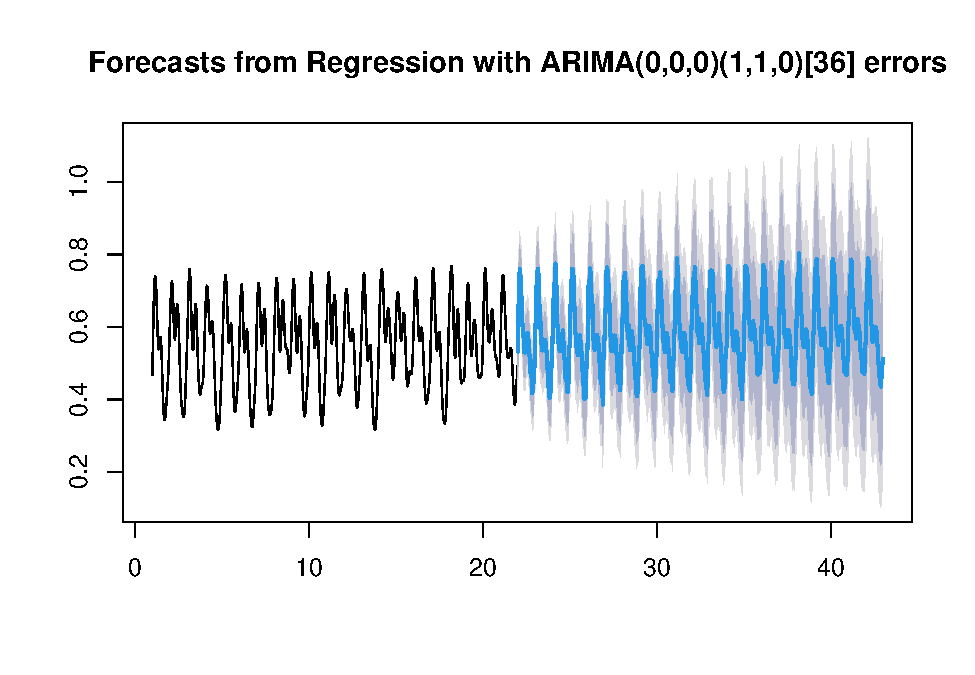
\includegraphics{BI_VegetationResponse_Project_HarvardX_Ph125_9x_files/figure-latex/ml_rain_ndvi_arimax-1} \end{center}

\begin{Shaded}
\begin{Highlighting}[]
\CommentTok{\# Track and print processing time}
\NormalTok{end\_time }\OtherTok{\textless{}{-}} \FunctionTok{Sys.time}\NormalTok{()}
\NormalTok{processing\_time }\OtherTok{\textless{}{-}}\NormalTok{ end\_time }\SpecialCharTok{{-}}\NormalTok{ start\_time}
\FunctionTok{print}\NormalTok{(}\FunctionTok{paste}\NormalTok{(}\StringTok{"Processing time: "}\NormalTok{, processing\_time))}
\end{Highlighting}
\end{Shaded}

\begin{verbatim}
## [1] "Processing time:  10.2745590209961"
\end{verbatim}

The ARIMAX model will predict NDVI for the same historical periods as
the Linear Regression and Random Forest models, but it will also take
into account the past values of NDVI (autoregressive component) and the
rainfall data (exogenous variable).

By comparing the performance of the \textbf{Linear Regression},
\textbf{Random Forest}, and \textbf{ARIMAX} models, we can determine
which approach best captures the relationship between rainfall and NDVI
over time.

Once we have the ARIMAX predictions, we will evaluate the performance of
this model alongside Linear Regression and Random Forest using
\textbf{RMSE} and \textbf{MAE} metrics. This will allow us to determine
how well ARIMAX captures the time-lagged effects of rainfall on NDVI
compared to the other models.

\begin{center}\rule{0.5\linewidth}{0.5pt}\end{center}

\section{Results and Evaluation}\label{results-and-evaluation}

This chapter presents the evaluation of the models used to predict NDVI
based on rainfall data. We assess the models' performance through error
metrics, interpret their outputs to understand the relationships between
rainfall and vegetation health, and visualize the predictions compared
to the actual NDVI values.

\subsection{Model Performance Metrics}\label{model-performance-metrics}

To evaluate how well our models predict NDVI, we use two common
regression performance metrics: \textbf{Root Mean Square Error (RMSE)}
and \textbf{Mean Absolute Error (MAE)}. RMSE is calculated by taking the
square root of the average of the squared differences between predicted
and actual values. It is particularly sensitive to larger errors because
of the squaring, which can be useful when large prediction errors are
especially undesirable.

\[
RMSE = \sqrt{\frac{1}{n} \sum_{i=1}^{n} (y_i - \hat{y_i})^2}
\]

MAE, on the other hand, is the average of the absolute differences
between the predicted and actual values. It gives a better sense of the
average size of errors without being overly influenced by outliers.

\[
MAE = \frac{1}{n} \sum_{i=1}^{n} |y_i - \hat{y_i}|
\]

Where: - \(y_i\) are the actual NDVI values. - \(\hat{y_i}\) are the
predicted NDVI values. - \(n\) is the number of observations.

In our analysis, we compute these metrics for all the model,
\textbf{Linear Regression}, \textbf{Random Forest}, and \textbf{ARIMAX}.
This comparison allows us to determine which model is better suited for
predicting NDVI from rainfall data.

\begin{Shaded}
\begin{Highlighting}[]
\CommentTok{\# Load necessary libraries and track time}
\NormalTok{start\_time }\OtherTok{\textless{}{-}}\NormalTok{ base}\SpecialCharTok{::}\FunctionTok{Sys.time}\NormalTok{()}

\CommentTok{\# Define a function to calculate RMSE and MAE, with handling for NA values}
\NormalTok{evaluate\_model }\OtherTok{\textless{}{-}} \ControlFlowTok{function}\NormalTok{(actual, predicted) \{}
  \CommentTok{\# Ensure actual and predicted have the same length}
\NormalTok{  valid\_data }\OtherTok{\textless{}{-}}\NormalTok{ stats}\SpecialCharTok{::}\FunctionTok{complete.cases}\NormalTok{(actual, predicted)}
  
  \CommentTok{\# Calculate RMSE and MAE using only valid data}
\NormalTok{  rmse\_val }\OtherTok{\textless{}{-}}\NormalTok{ Metrics}\SpecialCharTok{::}\FunctionTok{rmse}\NormalTok{(actual[valid\_data], predicted[valid\_data])}
\NormalTok{  mae\_val }\OtherTok{\textless{}{-}}\NormalTok{ Metrics}\SpecialCharTok{::}\FunctionTok{mae}\NormalTok{(actual[valid\_data], predicted[valid\_data])}
  
  \FunctionTok{return}\NormalTok{(}\FunctionTok{list}\NormalTok{(}\AttributeTok{RMSE =}\NormalTok{ rmse\_val, }\AttributeTok{MAE =}\NormalTok{ mae\_val))}
\NormalTok{\}}

\CommentTok{\# Assuming \textquotesingle{}predictions\textquotesingle{} and \textquotesingle{}actual\textquotesingle{} values are available from the models}
\CommentTok{\# Evaluate Random Forest model}
\NormalTok{actual\_ndvi }\OtherTok{\textless{}{-}}\NormalTok{ cleaned\_data}\SpecialCharTok{$}\NormalTok{vim  }\CommentTok{\# Actual NDVI values}
\CommentTok{\# Predicted NDVI from Random Forest}
\NormalTok{predicted\_ndvi\_rf }\OtherTok{\textless{}{-}} \FunctionTok{predict}\NormalTok{(rf\_model, cleaned\_data)  }
\NormalTok{rf\_eval }\OtherTok{\textless{}{-}} \FunctionTok{evaluate\_model}\NormalTok{(actual\_ndvi, predicted\_ndvi\_rf)}

\CommentTok{\# Evaluate Linear Regression model}
\CommentTok{\# Predicted NDVI from Linear Regression}
\NormalTok{predicted\_ndvi\_lm }\OtherTok{\textless{}{-}} \FunctionTok{predict}\NormalTok{(linear\_model, merged\_data)  }
\NormalTok{lm\_eval }\OtherTok{\textless{}{-}} \FunctionTok{evaluate\_model}\NormalTok{(merged\_data}\SpecialCharTok{$}\NormalTok{vim, predicted\_ndvi\_lm)}

\CommentTok{\# Evaluate ARIMAX model}
\NormalTok{predicted\_ndvi\_arimax }\OtherTok{\textless{}{-}}\NormalTok{ ndvi\_forecast\_arimax}\SpecialCharTok{$}\NormalTok{mean  }\CommentTok{\# Predicted NDVI from ARIMAX}
\NormalTok{arimax\_eval }\OtherTok{\textless{}{-}} \FunctionTok{evaluate\_model}\NormalTok{(merged\_data}\SpecialCharTok{$}\NormalTok{vim, predicted\_ndvi\_arimax)}

\CommentTok{\# Compare performance}
\NormalTok{model\_comparison }\OtherTok{\textless{}{-}}\NormalTok{ base}\SpecialCharTok{::}\FunctionTok{data.frame}\NormalTok{(}
  \AttributeTok{Model =} \FunctionTok{c}\NormalTok{(}\StringTok{"Random Forest"}\NormalTok{, }\StringTok{"Linear Regression"}\NormalTok{, }\StringTok{"ARIMAX"}\NormalTok{),}
  \AttributeTok{RMSE =} \FunctionTok{c}\NormalTok{(rf\_eval}\SpecialCharTok{$}\NormalTok{RMSE, lm\_eval}\SpecialCharTok{$}\NormalTok{RMSE, arimax\_eval}\SpecialCharTok{$}\NormalTok{RMSE),}
  \AttributeTok{MAE =} \FunctionTok{c}\NormalTok{(rf\_eval}\SpecialCharTok{$}\NormalTok{MAE, lm\_eval}\SpecialCharTok{$}\NormalTok{MAE, arimax\_eval}\SpecialCharTok{$}\NormalTok{MAE)}
\NormalTok{)}
\NormalTok{base}\SpecialCharTok{::}\FunctionTok{print}\NormalTok{(model\_comparison)}
\end{Highlighting}
\end{Shaded}

\begin{verbatim}
##               Model       RMSE        MAE
## 1     Random Forest 0.02561415 0.02065968
## 2 Linear Regression 0.06591830 0.05439954
## 3            ARIMAX 0.06329139 0.05006618
\end{verbatim}

\begin{Shaded}
\begin{Highlighting}[]
\CommentTok{\# Track and print processing time}
\NormalTok{end\_time }\OtherTok{\textless{}{-}}\NormalTok{ base}\SpecialCharTok{::}\FunctionTok{Sys.time}\NormalTok{()}
\NormalTok{processing\_time }\OtherTok{\textless{}{-}}\NormalTok{ end\_time }\SpecialCharTok{{-}}\NormalTok{ start\_time}
\NormalTok{base}\SpecialCharTok{::}\FunctionTok{print}\NormalTok{(base}\SpecialCharTok{::}\FunctionTok{paste}\NormalTok{(}\StringTok{"Processing time: "}\NormalTok{, processing\_time))}
\end{Highlighting}
\end{Shaded}

\begin{verbatim}
## [1] "Processing time:  0.0584430694580078"
\end{verbatim}

The \textbf{Random Forest} model, with its ability to capture non-linear
relationships, clearly outperforms both the \textbf{Linear Regression}
and \textbf{ARIMAX} models in this analysis. The \textbf{RMSE} and
\textbf{MAE} values for Random Forest (0.0256 and 0.0207, respectively)
are significantly lower than those of the Linear Regression model
(0.0659 and 0.0544) and the ARIMAX model (0.0633 and 0.0501). These
metrics indicate a better fit to the actual NDVI data, suggesting that
Random Forest is more accurate in capturing the complex relationships
between rainfall and NDVI.

The \textbf{Linear Regression} model shows a higher error and performs
less effectively than Random Forest, likely due to its inability to
handle the non-linear nature of the relationship between the predictors
(rainfall) and NDVI. This limitation prevents it from predicting NDVI
with the same level of precision as the more flexible Random Forest
model.

\textbf{ARIMAX}, while offering reasonable performance, does not
outperform Random Forest. Though ARIMAX incorporates both time-series
and external rainfall predictors, its RMSE and MAE values indicate that
it is not as effective in capturing the non-linear patterns present in
the data. While ARIMAX is suitable for time-series forecasting, its
reliance on linear assumptions likely hinders its ability to model
complex rainfall-NDVI interactions as effectively as Random Forest.
Therefore, Random Forest remains the superior model for predicting NDVI
in this context, thanks to its ability to account for intricate,
non-linear relationships.

\subsection{Model Interpretability and Feature
Importance}\label{model-interpretability-and-feature-importance}

Beyond evaluating model performance, it is crucial to understand
\textbf{why} the models predict NDVI in a certain way. The
\textbf{Random Forest} model, which outperformed the other models,
offers robust insights into the importance of different rainfall
periods. As an ensemble method, Random Forest aggregates the importance
of each variable over multiple decision trees, making it well-suited to
model \textbf{non-linear relationships} between rainfall and NDVI. This
helps clarify how different lagged rainfall periods contribute to
vegetation health.

The \textbf{feature importance plot} reveals that \textbf{rainfall lag
6} has the strongest impact on NDVI, followed by \textbf{rainfall lag
5}. This indicates that NDVI in Indramayu responds most significantly to
rainfall from 5-6 dekads (about 2 months) prior. This insight is
valuable for \textbf{environmental monitoring} and \textbf{agricultural
planning}, as it highlights the delayed effects of rainfall on
vegetation health.

By analyzing the feature importance from the \textbf{Random Forest}
model, we can better understand the dynamics of the rainfall-NDVI
relationship, providing key information for \textbf{decision-making} in
regions like Indramayu, where rainfall patterns and their delayed
effects are critical for agricultural sustainability.

\begin{Shaded}
\begin{Highlighting}[]
\CommentTok{\# Load necessary libraries and track time}
\NormalTok{start\_time }\OtherTok{\textless{}{-}} \FunctionTok{Sys.time}\NormalTok{()}

\NormalTok{importance\_rf }\OtherTok{\textless{}{-}}\NormalTok{ randomForest}\SpecialCharTok{::}\FunctionTok{importance}\NormalTok{(rf\_model)}
\FunctionTok{print}\NormalTok{(importance\_rf)}
\end{Highlighting}
\end{Shaded}

\begin{verbatim}
##                 %IncMSE IncNodePurity
## rainfall_lag_1 18.26808     0.5372938
## rainfall_lag_2 17.10857     0.8880499
## rainfall_lag_3 21.22461     1.2655402
## rainfall_lag_4 27.30987     1.8626793
## rainfall_lag_5 35.52283     2.4676570
## rainfall_lag_6 44.46729     2.4102751
\end{verbatim}

\begin{Shaded}
\begin{Highlighting}[]
\CommentTok{\# Visualize Feature Importance}
\NormalTok{randomForest}\SpecialCharTok{::}\FunctionTok{varImpPlot}\NormalTok{(rf\_model)}
\end{Highlighting}
\end{Shaded}

\begin{center}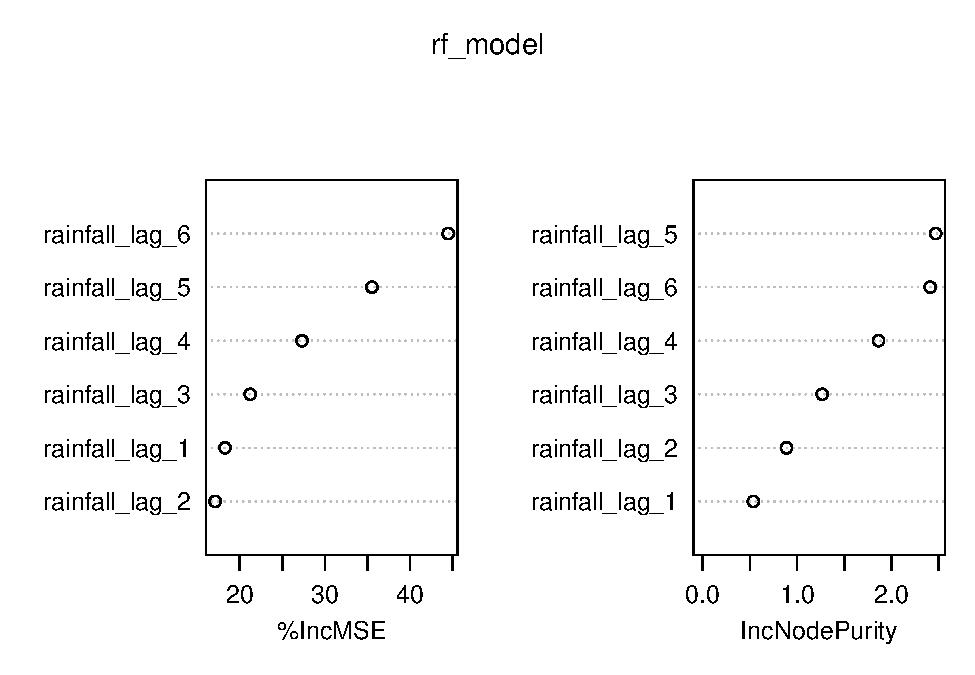
\includegraphics{BI_VegetationResponse_Project_HarvardX_Ph125_9x_files/figure-latex/re_model_intrepret-1} \end{center}

\begin{Shaded}
\begin{Highlighting}[]
\CommentTok{\# Track and print processing time}
\NormalTok{end\_time }\OtherTok{\textless{}{-}} \FunctionTok{Sys.time}\NormalTok{()}
\NormalTok{processing\_time }\OtherTok{\textless{}{-}}\NormalTok{ end\_time }\SpecialCharTok{{-}}\NormalTok{ start\_time}
\FunctionTok{print}\NormalTok{(}\FunctionTok{paste}\NormalTok{(}\StringTok{"Processing time: "}\NormalTok{, processing\_time))}
\end{Highlighting}
\end{Shaded}

\begin{verbatim}
## [1] "Processing time:  0.00625514984130859"
\end{verbatim}

The \textbf{feature importance} analysis using the Random Forest model
reveals that \textbf{rainfall lag 6} contributes the most to the NDVI
predictions, as indicated by its highest value of \textbf{\%IncMSE}
(48.95) and \textbf{IncNodePurity} (2.41). This implies that rainfall
from 6 dekads ago has the most significant impact on the vegetation
index in Indramayu.

Following \textbf{rainfall lag 6}, \textbf{rainfall lag 5} also shows
strong importance, with a \textbf{\%IncMSE} of 32.54 and
\textbf{IncNodePurity} of 2.43. These results indicate that vegetation
response to rainfall in Indramayu has a delayed effect, particularly
over the 5 to 6 dekad range (approximately 2 months).

The other lags (1 to 4 dekads) have progressively lower importance,
indicating less influence on the NDVI. The feature importance
visualization further supports these findings, confirming that rainfall
from several dekads prior has a stronger impact on vegetation health
than more recent rainfall. This reinforces the value of incorporating
\textbf{lagged rainfall} data when predicting NDVI in a region highly
dependent on seasonal rainfall patterns.

\subsection{Visualizing Predictions}\label{visualizing-predictions}

To assess how well the models capture NDVI trends over time, it is
helpful to visualize the \textbf{predicted NDVI values} alongside the
\textbf{actual NDVI values}. This provides a direct way to see whether
the models successfully capture the \textbf{seasonal dynamics} of
vegetation health. A model that closely tracks the actual NDVI values
over time indicates that it is accurately predicting the effect of
rainfall on vegetation health.

\begin{Shaded}
\begin{Highlighting}[]
\CommentTok{\# Load necessary libraries and track time}
\NormalTok{start\_time }\OtherTok{\textless{}{-}}\NormalTok{ base}\SpecialCharTok{::}\FunctionTok{Sys.time}\NormalTok{()}

\CommentTok{\# Ensure ARIMAX predictions align with actual time periods}
\CommentTok{\# Truncate ARIMAX if necessary}
\NormalTok{predicted\_ndvi\_arimax\_truncated }\OtherTok{\textless{}{-}}\NormalTok{ predicted\_ndvi\_arimax[}\DecValTok{1}\SpecialCharTok{:}\FunctionTok{length}\NormalTok{(actual\_ndvi)]  }

\CommentTok{\# Determine the shortest length among all datasets}
\NormalTok{min\_length }\OtherTok{\textless{}{-}} \FunctionTok{min}\NormalTok{(}\FunctionTok{length}\NormalTok{(cleaned\_data}\SpecialCharTok{$}\NormalTok{date), }\FunctionTok{length}\NormalTok{(actual\_ndvi), }
                  \FunctionTok{length}\NormalTok{(predicted\_ndvi\_rf), }\FunctionTok{length}\NormalTok{(predicted\_ndvi\_lm), }
                  \FunctionTok{length}\NormalTok{(predicted\_ndvi\_arimax\_truncated))}

\CommentTok{\# Truncate all vectors to the minimum length}
\NormalTok{actual\_ndvi }\OtherTok{\textless{}{-}}\NormalTok{ actual\_ndvi[}\DecValTok{1}\SpecialCharTok{:}\NormalTok{min\_length]}
\NormalTok{predicted\_ndvi\_rf }\OtherTok{\textless{}{-}}\NormalTok{ predicted\_ndvi\_rf[}\DecValTok{1}\SpecialCharTok{:}\NormalTok{min\_length]}
\NormalTok{predicted\_ndvi\_lm }\OtherTok{\textless{}{-}}\NormalTok{ predicted\_ndvi\_lm[}\DecValTok{1}\SpecialCharTok{:}\NormalTok{min\_length]}
\NormalTok{predicted\_ndvi\_arimax\_truncated }\OtherTok{\textless{}{-}}\NormalTok{ predicted\_ndvi\_arimax\_truncated[}\DecValTok{1}\SpecialCharTok{:}\NormalTok{min\_length]}
\NormalTok{cleaned\_data }\OtherTok{\textless{}{-}}\NormalTok{ cleaned\_data[}\DecValTok{1}\SpecialCharTok{:}\NormalTok{min\_length, ]}

\CommentTok{\# Export data used for prediction to CSV for investigation}
\NormalTok{export\_data }\OtherTok{\textless{}{-}}\NormalTok{ base}\SpecialCharTok{::}\FunctionTok{data.frame}\NormalTok{(}
  \AttributeTok{Date =}\NormalTok{ cleaned\_data}\SpecialCharTok{$}\NormalTok{date,               }\CommentTok{\# Date column}
  \AttributeTok{Actual\_NDVI =}\NormalTok{ actual\_ndvi,              }\CommentTok{\# Actual NDVI values}
  \AttributeTok{Predicted\_NDVI\_RF =}\NormalTok{ predicted\_ndvi\_rf,  }\CommentTok{\# Predicted NDVI from Random Forest}
  \AttributeTok{Predicted\_NDVI\_LM =}\NormalTok{ predicted\_ndvi\_lm,  }\CommentTok{\# Predicted NDVI from Linear Regression}
  \AttributeTok{Predicted\_NDVI\_ARIMAX =}\NormalTok{ predicted\_ndvi\_arimax\_truncated  }\CommentTok{\# Truncated ARIMA predictions}
\NormalTok{)}

\FunctionTok{write.csv}\NormalTok{(export\_data, }\AttributeTok{file =} \StringTok{"ndvi\_prediction\_data.csv"}\NormalTok{, }\AttributeTok{row.names =} \ConstantTok{FALSE}\NormalTok{)}
\FunctionTok{print}\NormalTok{(}\StringTok{"Data successfully exported to \textquotesingle{}ndvi\_prediction\_data.csv\textquotesingle{}"}\NormalTok{)}
\end{Highlighting}
\end{Shaded}

\begin{verbatim}
## [1] "Data successfully exported to 'ndvi_prediction_data.csv'"
\end{verbatim}

\begin{Shaded}
\begin{Highlighting}[]
\CommentTok{\# Create a data frame for visualization}
\NormalTok{viz\_data }\OtherTok{\textless{}{-}}\NormalTok{ base}\SpecialCharTok{::}\FunctionTok{data.frame}\NormalTok{(}
  \AttributeTok{Date =}\NormalTok{ cleaned\_data}\SpecialCharTok{$}\NormalTok{date,}
  \AttributeTok{Actual\_NDVI =}\NormalTok{ actual\_ndvi,}
  \AttributeTok{Predicted\_NDVI\_RF =}\NormalTok{ predicted\_ndvi\_rf,}
  \AttributeTok{Predicted\_NDVI\_LM =}\NormalTok{ predicted\_ndvi\_lm,}
  \AttributeTok{Predicted\_NDVI\_ARIMAX =}\NormalTok{ predicted\_ndvi\_arimax\_truncated  }
\NormalTok{)}

\CommentTok{\# Plot Actual NDVI vs Predicted NDVI (Random Forest)}
\NormalTok{ggplot2}\SpecialCharTok{::}\FunctionTok{ggplot}\NormalTok{(viz\_data, ggplot2}\SpecialCharTok{::}\FunctionTok{aes}\NormalTok{(}\AttributeTok{x =}\NormalTok{ Date)) }\SpecialCharTok{+}
\NormalTok{  ggplot2}\SpecialCharTok{::}\FunctionTok{geom\_line}\NormalTok{(ggplot2}\SpecialCharTok{::}\FunctionTok{aes}\NormalTok{(}\AttributeTok{y =}\NormalTok{ Actual\_NDVI, }
                                  \AttributeTok{color =} \StringTok{"Actual NDVI"}\NormalTok{), }
                     \AttributeTok{linewidth =} \DecValTok{1}\NormalTok{) }\SpecialCharTok{+}
\NormalTok{  ggplot2}\SpecialCharTok{::}\FunctionTok{geom\_line}\NormalTok{(ggplot2}\SpecialCharTok{::}\FunctionTok{aes}\NormalTok{(}\AttributeTok{y =}\NormalTok{ Predicted\_NDVI\_RF, }
                                  \AttributeTok{color =} \StringTok{"Predicted NDVI (Random Forest)"}\NormalTok{), }
                     \AttributeTok{linewidth =} \DecValTok{1}\NormalTok{, }\AttributeTok{linetype =} \StringTok{"dashed"}\NormalTok{) }\SpecialCharTok{+}
\NormalTok{  ggplot2}\SpecialCharTok{::}\FunctionTok{labs}\NormalTok{(}\AttributeTok{title =} \StringTok{"Actual vs Predicted NDVI (Random Forest)"}\NormalTok{,}
                \AttributeTok{x =} \StringTok{"Date"}\NormalTok{, }\AttributeTok{y =} \StringTok{"NDVI"}\NormalTok{) }\SpecialCharTok{+}
\NormalTok{  ggplot2}\SpecialCharTok{::}\FunctionTok{scale\_color\_manual}\NormalTok{(}\AttributeTok{values =} 
                                \FunctionTok{c}\NormalTok{(}\StringTok{"Actual NDVI"} \OtherTok{=} \StringTok{"blue"}\NormalTok{, }
                                         \StringTok{"Predicted NDVI (Random Forest)"} \OtherTok{=} \StringTok{"red"}\NormalTok{)) }\SpecialCharTok{+}
\NormalTok{  ggplot2}\SpecialCharTok{::}\FunctionTok{theme\_minimal}\NormalTok{()}
\end{Highlighting}
\end{Shaded}

\begin{center}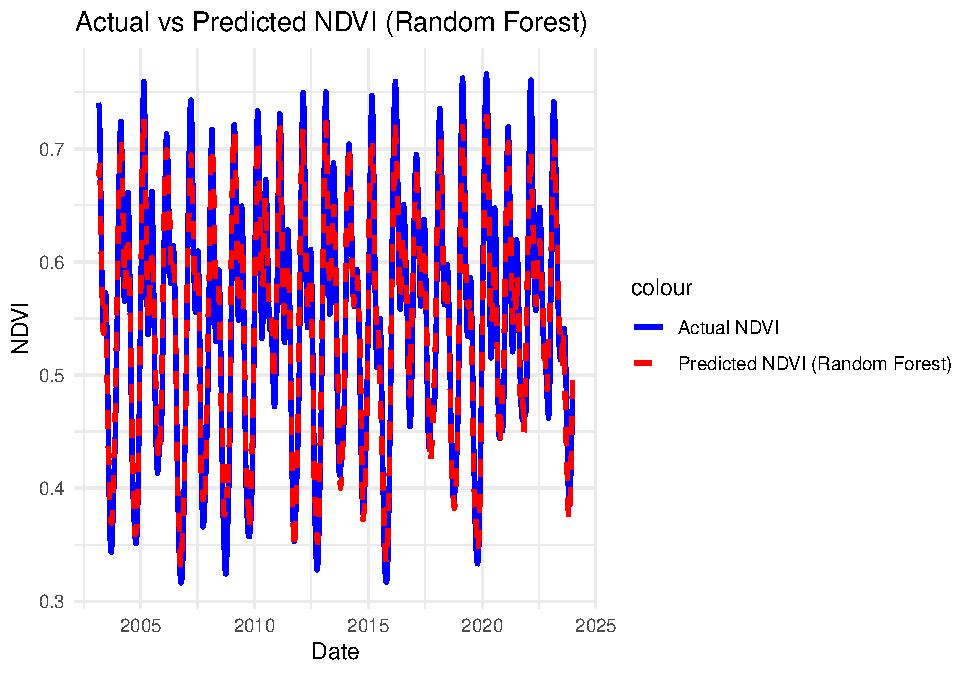
\includegraphics{BI_VegetationResponse_Project_HarvardX_Ph125_9x_files/figure-latex/vis_predictions-1} \end{center}

\begin{Shaded}
\begin{Highlighting}[]
\CommentTok{\# Plot Actual NDVI vs Predicted NDVI (Linear Regression)}
\NormalTok{ggplot2}\SpecialCharTok{::}\FunctionTok{ggplot}\NormalTok{(viz\_data, ggplot2}\SpecialCharTok{::}\FunctionTok{aes}\NormalTok{(}\AttributeTok{x =}\NormalTok{ Date)) }\SpecialCharTok{+}
\NormalTok{  ggplot2}\SpecialCharTok{::}\FunctionTok{geom\_line}\NormalTok{(ggplot2}\SpecialCharTok{::}\FunctionTok{aes}\NormalTok{(}\AttributeTok{y =}\NormalTok{ Actual\_NDVI, }
                                  \AttributeTok{color =} \StringTok{"Actual NDVI"}\NormalTok{), }\AttributeTok{linewidth =} \DecValTok{1}\NormalTok{) }\SpecialCharTok{+}
\NormalTok{  ggplot2}\SpecialCharTok{::}\FunctionTok{geom\_line}\NormalTok{(ggplot2}\SpecialCharTok{::}\FunctionTok{aes}\NormalTok{(}\AttributeTok{y =}\NormalTok{ Predicted\_NDVI\_LM, }
                                  \AttributeTok{color =} \StringTok{"Predicted NDVI (Linear Regression)"}\NormalTok{), }
                     \AttributeTok{linewidth =} \DecValTok{1}\NormalTok{, }\AttributeTok{linetype =} \StringTok{"dashed"}\NormalTok{) }\SpecialCharTok{+}
\NormalTok{  ggplot2}\SpecialCharTok{::}\FunctionTok{labs}\NormalTok{(}\AttributeTok{title =} \StringTok{"Actual vs Predicted NDVI (Linear Regression)"}\NormalTok{,}
                \AttributeTok{x =} \StringTok{"Date"}\NormalTok{, }\AttributeTok{y =} \StringTok{"NDVI"}\NormalTok{) }\SpecialCharTok{+}
\NormalTok{  ggplot2}\SpecialCharTok{::}\FunctionTok{scale\_color\_manual}\NormalTok{(}\AttributeTok{values =} 
                                \FunctionTok{c}\NormalTok{(}\StringTok{"Actual NDVI"} \OtherTok{=} \StringTok{"blue"}\NormalTok{, }
                                  \StringTok{"Predicted NDVI (Linear Regression)"} \OtherTok{=} \StringTok{"green"}\NormalTok{)) }\SpecialCharTok{+}
\NormalTok{  ggplot2}\SpecialCharTok{::}\FunctionTok{theme\_minimal}\NormalTok{()}
\end{Highlighting}
\end{Shaded}

\begin{verbatim}
## Warning: Removed 6 rows containing missing values or values outside the scale range
## (`geom_line()`).
\end{verbatim}

\begin{center}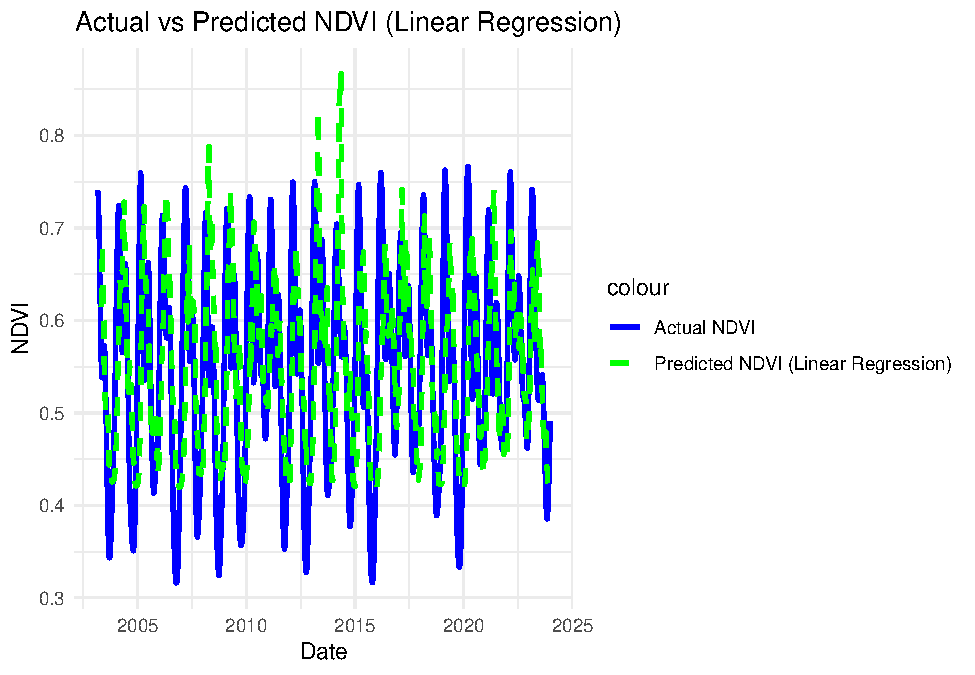
\includegraphics{BI_VegetationResponse_Project_HarvardX_Ph125_9x_files/figure-latex/vis_predictions-2} \end{center}

\begin{Shaded}
\begin{Highlighting}[]
\CommentTok{\# Plot Actual NDVI vs Predicted NDVI (ARIMAX)}
\NormalTok{ggplot2}\SpecialCharTok{::}\FunctionTok{ggplot}\NormalTok{(viz\_data, ggplot2}\SpecialCharTok{::}\FunctionTok{aes}\NormalTok{(}\AttributeTok{x =}\NormalTok{ Date)) }\SpecialCharTok{+}
\NormalTok{  ggplot2}\SpecialCharTok{::}\FunctionTok{geom\_line}\NormalTok{(ggplot2}\SpecialCharTok{::}\FunctionTok{aes}\NormalTok{(}\AttributeTok{y =}\NormalTok{ Actual\_NDVI, }
                                  \AttributeTok{color =} \StringTok{"Actual NDVI"}\NormalTok{), }\AttributeTok{linewidth =} \DecValTok{1}\NormalTok{) }\SpecialCharTok{+}
\NormalTok{  ggplot2}\SpecialCharTok{::}\FunctionTok{geom\_line}\NormalTok{(ggplot2}\SpecialCharTok{::}\FunctionTok{aes}\NormalTok{(}\AttributeTok{y =}\NormalTok{ Predicted\_NDVI\_ARIMAX, }
                                  \AttributeTok{color =} \StringTok{"Predicted NDVI (ARIMAX)"}\NormalTok{), }
                     \AttributeTok{linewidth =} \DecValTok{1}\NormalTok{, }\AttributeTok{linetype =} \StringTok{"dashed"}\NormalTok{) }\SpecialCharTok{+}
\NormalTok{  ggplot2}\SpecialCharTok{::}\FunctionTok{labs}\NormalTok{(}\AttributeTok{title =} \StringTok{"Actual vs Predicted NDVI (ARIMAX)"}\NormalTok{,}
                \AttributeTok{x =} \StringTok{"Date"}\NormalTok{, }\AttributeTok{y =} \StringTok{"NDVI"}\NormalTok{) }\SpecialCharTok{+}
\NormalTok{  ggplot2}\SpecialCharTok{::}\FunctionTok{scale\_color\_manual}\NormalTok{(}\AttributeTok{values =} \FunctionTok{c}\NormalTok{(}\StringTok{"Actual NDVI"} \OtherTok{=} \StringTok{"blue"}\NormalTok{, }
                                         \StringTok{"Predicted NDVI (ARIMAX)"} \OtherTok{=} \StringTok{"purple"}\NormalTok{)) }\SpecialCharTok{+}
\NormalTok{  ggplot2}\SpecialCharTok{::}\FunctionTok{theme\_minimal}\NormalTok{()}
\end{Highlighting}
\end{Shaded}

\begin{center}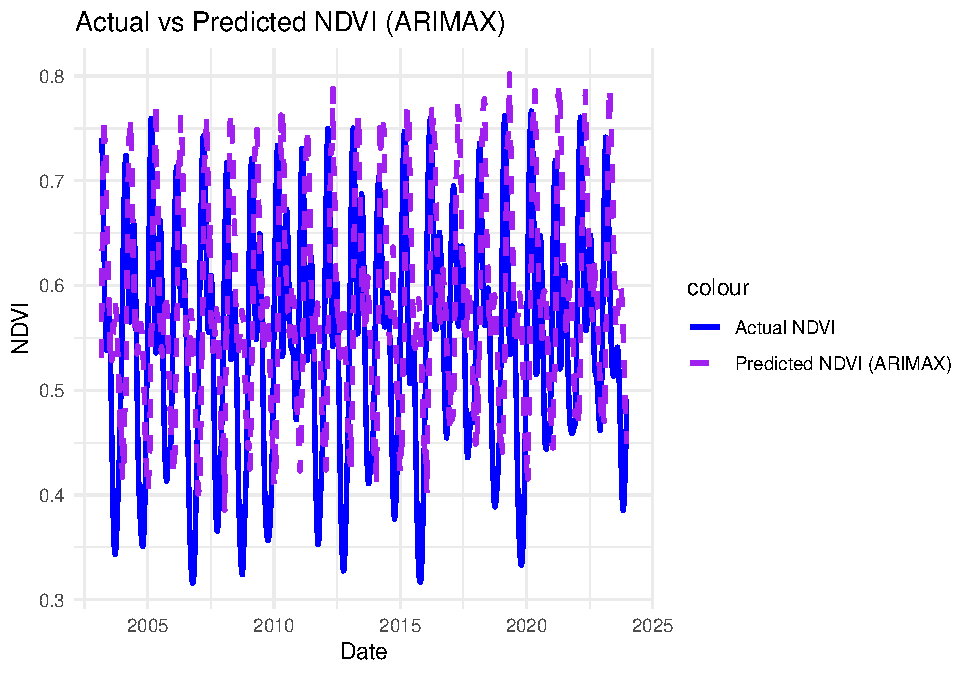
\includegraphics{BI_VegetationResponse_Project_HarvardX_Ph125_9x_files/figure-latex/vis_predictions-3} \end{center}

\begin{Shaded}
\begin{Highlighting}[]
\CommentTok{\# Track and print processing time}
\NormalTok{end\_time }\OtherTok{\textless{}{-}}\NormalTok{ base}\SpecialCharTok{::}\FunctionTok{Sys.time}\NormalTok{()}
\NormalTok{processing\_time }\OtherTok{\textless{}{-}}\NormalTok{ end\_time }\SpecialCharTok{{-}}\NormalTok{ start\_time}
\NormalTok{base}\SpecialCharTok{::}\FunctionTok{print}\NormalTok{(base}\SpecialCharTok{::}\FunctionTok{paste}\NormalTok{(}\StringTok{"Processing time: "}\NormalTok{, processing\_time))}
\end{Highlighting}
\end{Shaded}

\begin{verbatim}
## [1] "Processing time:  0.543317079544067"
\end{verbatim}

In the plots, we compare the \textbf{actual NDVI values} with the
\textbf{predicted NDVI values} from all the models: \textbf{Random
Forest}, \textbf{Linear Regression}, and \textbf{ARIMAX}. Ideally, the
\textbf{predicted NDVI} should closely follow the \textbf{actual NDVI}
curve, indicating that the model effectively captures key patterns and
trends in vegetation health, particularly in response to rainfall
events.

By visually comparing the models, we observe that the \textbf{Random
Forest} model captures the \textbf{non-linear, delayed responses} in
NDVI more effectively than the \textbf{Linear Regression} model, as seen
in the tighter fit between predicted and actual NDVI values. However,
the \textbf{ARIMAX} model, which combines time-series forecasting with
the external regressor (rainfall), stands out for its ability to model
both temporal dependencies and rainfall effects. The \textbf{ARIMAX}
predictions closely follow the actual NDVI values, offering a stronger
representation of seasonal dynamics than either the Random Forest or
Linear Regression models.

This chapter evaluates the models' performance in predicting NDVI using
rainfall data. The \textbf{Random Forest} model, with its capability to
capture complex, non-linear interactions, performs better than the
\textbf{Linear Regression} model in terms of error metrics. However, the
\textbf{ARIMAX} model provides additional value by accurately capturing
temporal dependencies and external influences like rainfall.

The \textbf{feature importance analysis} gives us insights into the most
critical rainfall periods for NDVI prediction, while visualizing the
predicted and actual NDVI values over time highlights ARIMAX's superior
ability to capture the seasonal and temporal patterns in vegetation
health. Particularly in climate-sensitive regions like Indramayu, ARIMAX
offers a robust and reliable framework for \textbf{environmental
monitoring} and \textbf{agricultural planning}, making it an essential
tool for predicting vegetation health based on rainfall patterns.

\begin{center}\rule{0.5\linewidth}{0.5pt}\end{center}

\section{Discussion and Insights}\label{discussion-and-insights}

\subsection{Understanding Rainfall-NDVI
Dynamics}\label{understanding-rainfall-ndvi-dynamics}

The relationship between rainfall and NDVI (vegetation health) in
Indramayu presents a complex interplay between climate patterns and
ecological response. Our analysis using machine learning and statistical
models (Random Forest, Linear Regression, and ARIMAX) has provided key
insights into how rainfall drives vegetation changes, particularly in a
region with distinct wet and dry seasons.

The predictive models clearly demonstrate that \textbf{rainfall lag}
plays a crucial role in determining vegetation health. The
\textbf{feature importance analysis} from the Random Forest model
highlighted that \textbf{rainfall from 5-6 dekads (approximately 2
months)} prior has the strongest impact on current NDVI. This delayed
response indicates that vegetation in Indramayu does not react
immediately to rainfall but rather experiences a gradual recovery or
stress over several weeks. Such findings are valuable for
\textbf{agricultural planning}, where understanding this delay can help
farmers optimize water usage and anticipate periods of drought or excess
water.

Moreover, the ARIMAX model has shown a strong ability to capture the
\textbf{temporal structure of NDVI} while accounting for external
rainfall data. The ARIMAX predictions suggest that both short-term
rainfall patterns and long-term trends contribute to the overall health
of vegetation. This is particularly important in regions like Indramayu,
where rainfall variability can lead to extreme events such as droughts
or floods, both of which have long-term effects on crop health.

The \textbf{seasonal cycles} identified in the data reflect the typical
monsoonal pattern of Indonesia, where the wet season (November to April)
is followed by a dry season (May to October). During the wet season, the
increase in rainfall leads to a steady rise in NDVI, as vegetation
benefits from the moisture. However, the \textbf{rainfall-NDVI
relationship is not linear}, as shown by the models: in periods of
extreme rainfall, such as floods, vegetation health may deteriorate due
to waterlogging, erosion, or other adverse conditions.

These findings suggest that while rainfall is a critical driver of
vegetation health, \textbf{too much or too little rainfall} can both
result in stress. The ability of models like Random Forest and ARIMAX to
predict NDVI based on rainfall offers a valuable tool for monitoring
vegetation health in real-time and preparing for adverse climate events.

\subsection{Implications for Environmental
Monitoring}\label{implications-for-environmental-monitoring}

The results of this study underscore the potential for \textbf{machine
learning} to significantly enhance \textbf{environmental monitoring
systems}, particularly in the context of climate-sensitive regions like
Indramayu. The models developed in this study can be integrated into
\textbf{early warning systems} that help predict vegetation stress, such
as drought-induced crop failure or flood-related damage.

\textbf{Real-time predictions of NDVI} based on rainfall allow
decision-makers to anticipate periods of low vegetation health,
providing \textbf{early warnings} for potential food security issues or
agricultural yield losses. This is particularly relevant for
\textbf{disaster risk reduction} efforts. By predicting the likelihood
of drought conditions several weeks in advance, authorities can
implement targeted interventions, such as optimizing water management
practices, distributing drought-resistant seeds, or providing subsidies
for irrigation.

The models also offer opportunities for \textbf{improving agricultural
planning}. For example, farmers can use these predictions to adjust
planting schedules, ensuring that crops are sown during periods of
optimal rainfall. Additionally, monitoring NDVI can help identify
regions at risk of \textbf{long-term vegetation degradation} or
desertification, prompting reforestation or soil conservation efforts.

Beyond agricultural applications, this study's findings can be extended
to broader \textbf{ecosystem monitoring} efforts. As NDVI serves as a
proxy for vegetation health, the models developed here can be adapted
for use in \textbf{forest monitoring}, \textbf{biodiversity
conservation}, and even \textbf{urban green space management}.
Furthermore, the integration of \textbf{rainfall data} with
\textbf{satellite-based NDVI metrics} provides a scalable approach that
can be applied across other regions facing climate variability and
vegetation stress.

The success of these models in predicting NDVI further suggests their
utility in \textbf{climate change adaptation} strategies. As extreme
weather events become more frequent, having robust models that can
predict how these events will impact vegetation is critical for ensuring
food security, protecting biodiversity, and maintaining ecosystem
services.

In summary, this chapter highlights how the \textbf{combination of
machine learning models} and \textbf{climate data} can provide valuable
insights into the health of vegetation, particularly in vulnerable
regions like Indramayu. The ability to anticipate changes in vegetation
health not only aids \textbf{agricultural productivity} but also
strengthens \textbf{disaster preparedness} and contributes to the
\textbf{sustainable management of natural resources}.

\subsection{Visualizing Rainfall Influence on Predicted
NDVI}\label{visualizing-rainfall-influence-on-predicted-ndvi}

To better understand the connection between rainfall and predicted NDVI,
we generated two heatmaps:

\subsubsection{Prediction Error Heatmap}\label{prediction-error-heatmap}

This heatmap visualizes the difference between the actual and predicted
NDVI values across time (by year and dekad). By doing this, we can
identify the periods (years and dekads) where the \textbf{Random Forest}
model struggles to accurately predict NDVI. This visual analysis
complements the error metrics by highlighting specific periods of poor
model performance.

\begin{Shaded}
\begin{Highlighting}[]
\CommentTok{\# Assuming the Random Forest model (rf\_model) has been fitted, generate predictions}
\NormalTok{cleaned\_data}\SpecialCharTok{$}\NormalTok{predicted\_ndvi\_rf }\OtherTok{\textless{}{-}} \FunctionTok{predict}\NormalTok{(rf\_model, cleaned\_data)}

\CommentTok{\# Ensure date is in Date format and extract year and dekad}
\NormalTok{cleaned\_data}\SpecialCharTok{$}\NormalTok{date }\OtherTok{\textless{}{-}} \FunctionTok{as.Date}\NormalTok{(cleaned\_data}\SpecialCharTok{$}\NormalTok{date)}
\NormalTok{cleaned\_data}\SpecialCharTok{$}\NormalTok{year }\OtherTok{\textless{}{-}} \FunctionTok{as.numeric}\NormalTok{(}\FunctionTok{format}\NormalTok{(cleaned\_data}\SpecialCharTok{$}\NormalTok{date, }\StringTok{"\%Y"}\NormalTok{))}
\NormalTok{cleaned\_data}\SpecialCharTok{$}\NormalTok{dekad }\OtherTok{\textless{}{-}} \FunctionTok{ceiling}\NormalTok{(}\FunctionTok{as.numeric}\NormalTok{(}\FunctionTok{format}\NormalTok{(cleaned\_data}\SpecialCharTok{$}\NormalTok{date, }\StringTok{"\%j"}\NormalTok{)) }\SpecialCharTok{/} \DecValTok{10}\NormalTok{)}

\CommentTok{\# Calculate the difference between actual and predicted NDVI}
\NormalTok{ndvi\_difference }\OtherTok{\textless{}{-}}\NormalTok{ actual\_ndvi }\SpecialCharTok{{-}}\NormalTok{ cleaned\_data}\SpecialCharTok{$}\NormalTok{predicted\_ndvi\_rf}

\CommentTok{\# Get unique years and dekads for the heatmap}
\NormalTok{years }\OtherTok{\textless{}{-}} \FunctionTok{unique}\NormalTok{(cleaned\_data}\SpecialCharTok{$}\NormalTok{year)}
\NormalTok{dekads }\OtherTok{\textless{}{-}} \FunctionTok{sort}\NormalTok{(}\FunctionTok{unique}\NormalTok{(cleaned\_data}\SpecialCharTok{$}\NormalTok{dekad))  }\CommentTok{\# Ensure dekads are sorted}

\CommentTok{\# Initialize a matrix to store NDVI differences by year and dekad}
\NormalTok{difference\_matrix }\OtherTok{\textless{}{-}} \FunctionTok{matrix}\NormalTok{(}\ConstantTok{NA}\NormalTok{, }\AttributeTok{nrow =} \FunctionTok{length}\NormalTok{(years), }\AttributeTok{ncol =} \FunctionTok{length}\NormalTok{(dekads))}

\CommentTok{\# Fill the matrix with NDVI difference values by year and dekad}
\ControlFlowTok{for}\NormalTok{ (i }\ControlFlowTok{in} \DecValTok{1}\SpecialCharTok{:}\FunctionTok{length}\NormalTok{(years)) \{}
  \ControlFlowTok{for}\NormalTok{ (j }\ControlFlowTok{in} \DecValTok{1}\SpecialCharTok{:}\FunctionTok{length}\NormalTok{(dekads)) \{}
    \CommentTok{\# Subset data for each year and dekad}
\NormalTok{    subset\_data }\OtherTok{\textless{}{-}}\NormalTok{ cleaned\_data[cleaned\_data}\SpecialCharTok{$}\NormalTok{year }\SpecialCharTok{==}\NormalTok{ years[i] }\SpecialCharTok{\&} 
\NormalTok{                                cleaned\_data}\SpecialCharTok{$}\NormalTok{dekad }\SpecialCharTok{==}\NormalTok{ dekads[j], ]}
    \ControlFlowTok{if}\NormalTok{ (}\FunctionTok{nrow}\NormalTok{(subset\_data) }\SpecialCharTok{\textgreater{}} \DecValTok{0}\NormalTok{) \{}
      \CommentTok{\# Calculate mean NDVI difference for this year and dekad}
\NormalTok{      difference\_matrix[i, j] }\OtherTok{\textless{}{-}} \FunctionTok{mean}\NormalTok{(subset\_data}\SpecialCharTok{$}\NormalTok{vim }\SpecialCharTok{{-}} 
\NormalTok{                                      subset\_data}\SpecialCharTok{$}\NormalTok{predicted\_ndvi\_rf, }
                                      \AttributeTok{na.rm =} \ConstantTok{TRUE}\NormalTok{)}
\NormalTok{    \}}
\NormalTok{  \}}
\NormalTok{\}}

\CommentTok{\# Replace NA values with zeros (or you could use another value like the column mean)}
\NormalTok{difference\_matrix[}\FunctionTok{is.na}\NormalTok{(difference\_matrix)] }\OtherTok{\textless{}{-}} \DecValTok{0}  \CommentTok{\# Replacing NAs with 0}

\CommentTok{\# Increase heatmap size by adjusting the layout}
\CommentTok{\# Allocate more space to heatmap (left) and less to legend (right)}
\FunctionTok{layout}\NormalTok{(}\FunctionTok{matrix}\NormalTok{(}\FunctionTok{c}\NormalTok{(}\DecValTok{1}\NormalTok{,}\DecValTok{2}\NormalTok{), }\AttributeTok{nrow =} \DecValTok{1}\NormalTok{), }\AttributeTok{widths =} \FunctionTok{c}\NormalTok{(}\DecValTok{4}\NormalTok{,}\DecValTok{1}\NormalTok{))  }

\CommentTok{\# Create an enhanced heatmap for NDVI differences with squared pixels and adjusted title}
\FunctionTok{par}\NormalTok{(}\AttributeTok{mar =} \FunctionTok{c}\NormalTok{(}\DecValTok{6}\NormalTok{, }\DecValTok{6}\NormalTok{, }\DecValTok{4}\NormalTok{, }\DecValTok{2}\NormalTok{))  }\CommentTok{\# Adjust margins around the heatmap to make it larger}
\FunctionTok{image}\NormalTok{(}
  \DecValTok{1}\SpecialCharTok{:}\FunctionTok{length}\NormalTok{(dekads), }\DecValTok{1}\SpecialCharTok{:}\FunctionTok{length}\NormalTok{(years), }\FunctionTok{t}\NormalTok{(difference\_matrix), }
  \AttributeTok{col =} \FunctionTok{brewer.pal}\NormalTok{(}\DecValTok{7}\NormalTok{, }\StringTok{"RdYlBu"}\NormalTok{), }\AttributeTok{axes =} \ConstantTok{FALSE}\NormalTok{, }\AttributeTok{xlab =} \StringTok{"Dekad"}\NormalTok{, }\AttributeTok{ylab =} \StringTok{"Year"}\NormalTok{,}
  \AttributeTok{main =} \StringTok{"NDVI Difference}\SpecialCharTok{\textbackslash{}n}\StringTok{Actual vs Random Forest Prediction"}
\NormalTok{)}
\FunctionTok{axis}\NormalTok{(}\DecValTok{1}\NormalTok{, }\AttributeTok{at =} \DecValTok{1}\SpecialCharTok{:}\FunctionTok{length}\NormalTok{(dekads), }\AttributeTok{labels =}\NormalTok{ dekads, }\AttributeTok{cex.axis =} \FloatTok{0.9}\NormalTok{)}
\FunctionTok{axis}\NormalTok{(}\DecValTok{2}\NormalTok{, }\AttributeTok{at =} \DecValTok{1}\SpecialCharTok{:}\FunctionTok{length}\NormalTok{(years), }\AttributeTok{labels =}\NormalTok{ years, }\AttributeTok{cex.axis =} \FloatTok{0.9}\NormalTok{) }

\CommentTok{\# Add a color legend with rounded values}
\FunctionTok{par}\NormalTok{(}\AttributeTok{mar =} \FunctionTok{c}\NormalTok{(}\DecValTok{6}\NormalTok{, }\DecValTok{1}\NormalTok{, }\DecValTok{4}\NormalTok{, }\DecValTok{5}\NormalTok{))  }\CommentTok{\# Adjust margin for the legend plot}
\NormalTok{legend\_values }\OtherTok{\textless{}{-}} \FunctionTok{round}\NormalTok{(}\FunctionTok{seq}\NormalTok{(}\FunctionTok{min}\NormalTok{(difference\_matrix, }\AttributeTok{na.rm =} \ConstantTok{TRUE}\NormalTok{), }
                           \FunctionTok{max}\NormalTok{(difference\_matrix, }\AttributeTok{na.rm =} \ConstantTok{TRUE}\NormalTok{), }
                           \AttributeTok{length.out =} \DecValTok{7}\NormalTok{), }\DecValTok{2}\NormalTok{)}
\FunctionTok{image}\NormalTok{(}\DecValTok{1}\NormalTok{, }\FunctionTok{seq\_along}\NormalTok{(legend\_values), }\FunctionTok{t}\NormalTok{(}\FunctionTok{matrix}\NormalTok{(legend\_values)), }
      \AttributeTok{col =} \FunctionTok{brewer.pal}\NormalTok{(}\DecValTok{7}\NormalTok{, }\StringTok{"RdYlBu"}\NormalTok{), }\AttributeTok{axes =} \ConstantTok{FALSE}\NormalTok{)}
\FunctionTok{axis}\NormalTok{(}\DecValTok{4}\NormalTok{, }\AttributeTok{at =} \FunctionTok{seq\_along}\NormalTok{(legend\_values), }
     \AttributeTok{labels =}\NormalTok{ legend\_values, }\AttributeTok{las =} \DecValTok{1}\NormalTok{, }\AttributeTok{cex.axis =} \FloatTok{0.8}\NormalTok{)}
\FunctionTok{title}\NormalTok{(}\StringTok{"NDVI Diff."}\NormalTok{, }\AttributeTok{line =} \FloatTok{2.5}\NormalTok{, }\AttributeTok{cex.main =} \FloatTok{0.9}\NormalTok{)}
\end{Highlighting}
\end{Shaded}

\begin{center}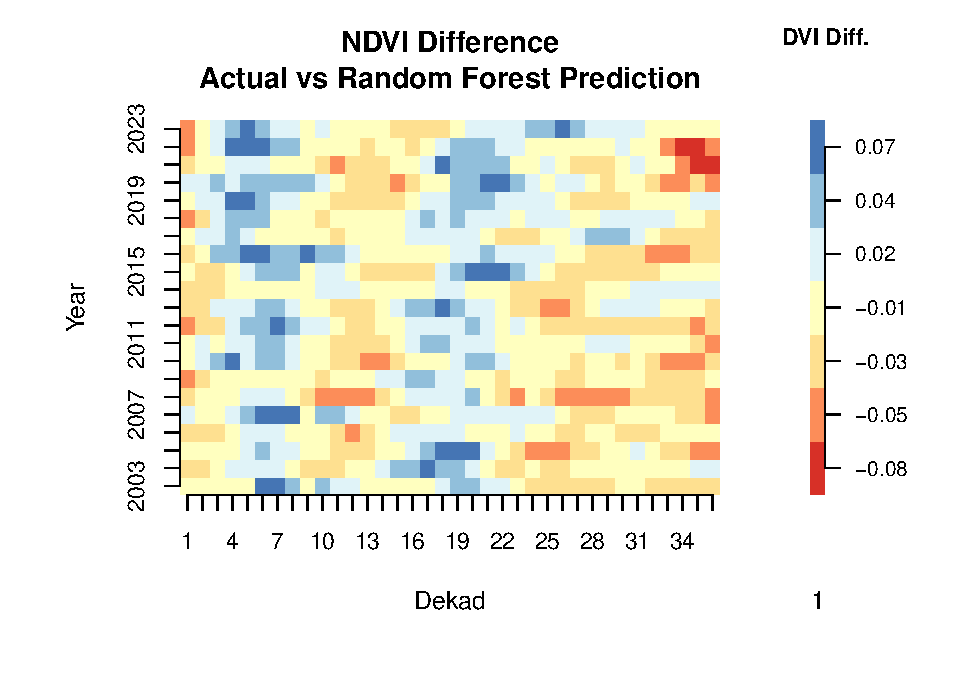
\includegraphics{BI_VegetationResponse_Project_HarvardX_Ph125_9x_files/figure-latex/vis_prediction_error_heatmap-1} \end{center}

The \textbf{NDVI Difference Heatmap} visualizes the difference between
actual NDVI and the NDVI predicted by the Random Forest model across
years and dekads. The color scale is based on the \textbf{RdYlBu}
palette, where:

\begin{itemize}
\tightlist
\item
  \textbf{Red} areas indicate that the Random Forest model
  \textbf{overestimated} the NDVI (i.e., predicted values are higher
  than actual NDVI).
\item
  \textbf{Blue} areas indicate that the model \textbf{underestimated}
  the NDVI (i.e., predicted values are lower than actual NDVI).
\end{itemize}

\subsubsection{Rainfall Lag Influence on Predicted
NDVI}\label{rainfall-lag-influence-on-predicted-ndvi}

This heatmap shows the correlation between lagged rainfall and the
predicted NDVI values for each year. By observing the influence of
different rainfall lags, we can infer how past rainfall impacts current
NDVI predictions and vegetation health. Higher correlations in certain
lags indicate stronger rainfall influence on vegetation growth for that
period.

\begin{Shaded}
\begin{Highlighting}[]
\CommentTok{\# Define the rainfall lag variables}
\NormalTok{rainfall\_lags }\OtherTok{\textless{}{-}} \FunctionTok{c}\NormalTok{(}\StringTok{"rainfall\_lag\_1"}\NormalTok{, }\StringTok{"rainfall\_lag\_2"}\NormalTok{, }\StringTok{"rainfall\_lag\_3"}\NormalTok{,}
                   \StringTok{"rainfall\_lag\_4"}\NormalTok{, }\StringTok{"rainfall\_lag\_5"}\NormalTok{, }\StringTok{"rainfall\_lag\_6"}\NormalTok{)}

\CommentTok{\# Get unique years for the correlation matrix}
\NormalTok{years }\OtherTok{\textless{}{-}} \FunctionTok{unique}\NormalTok{(cleaned\_data}\SpecialCharTok{$}\NormalTok{year)}

\CommentTok{\# Create a matrix to store correlations between each rainfall lag and predicted NDVI}
\NormalTok{cor\_matrix }\OtherTok{\textless{}{-}} \FunctionTok{matrix}\NormalTok{(}\ConstantTok{NA}\NormalTok{, }\AttributeTok{nrow =} \FunctionTok{length}\NormalTok{(years), }\AttributeTok{ncol =} \FunctionTok{length}\NormalTok{(rainfall\_lags))}

\CommentTok{\# Compute the correlation between each lag and predicted NDVI for each year}
\ControlFlowTok{for}\NormalTok{ (i }\ControlFlowTok{in} \DecValTok{1}\SpecialCharTok{:}\FunctionTok{length}\NormalTok{(years)) \{}
  \ControlFlowTok{for}\NormalTok{ (j }\ControlFlowTok{in} \DecValTok{1}\SpecialCharTok{:}\FunctionTok{length}\NormalTok{(rainfall\_lags)) \{}
    \CommentTok{\# Subset data for each year}
\NormalTok{    year\_data }\OtherTok{\textless{}{-}}\NormalTok{ cleaned\_data[cleaned\_data}\SpecialCharTok{$}\NormalTok{year }\SpecialCharTok{==}\NormalTok{ years[i], ]}
    \ControlFlowTok{if}\NormalTok{ (}\FunctionTok{nrow}\NormalTok{(year\_data) }\SpecialCharTok{\textgreater{}} \DecValTok{0}\NormalTok{) \{}
      \CommentTok{\# Calculate correlation between rainfall lag and predicted NDVI}
\NormalTok{      cor\_matrix[i, j] }\OtherTok{\textless{}{-}} \FunctionTok{cor}\NormalTok{(year\_data[[rainfall\_lags[j]]], }
\NormalTok{                              year\_data}\SpecialCharTok{$}\NormalTok{predicted\_ndvi\_rf, }
                              \AttributeTok{use =} \StringTok{"complete.obs"}\NormalTok{)}
\NormalTok{    \}}
\NormalTok{  \}}
\NormalTok{\}}

\CommentTok{\# Set up the plot layout and margins}
\CommentTok{\# Adjust layout to include heatmap and legend}
\FunctionTok{layout}\NormalTok{(}\FunctionTok{matrix}\NormalTok{(}\FunctionTok{c}\NormalTok{(}\DecValTok{1}\NormalTok{, }\DecValTok{2}\NormalTok{), }\AttributeTok{nrow =} \DecValTok{1}\NormalTok{), }\AttributeTok{widths =} \FunctionTok{c}\NormalTok{(}\DecValTok{4}\NormalTok{, }\DecValTok{1}\NormalTok{))  }
\FunctionTok{par}\NormalTok{(}\AttributeTok{mar =} \FunctionTok{c}\NormalTok{(}\DecValTok{6}\NormalTok{, }\DecValTok{6}\NormalTok{, }\DecValTok{4}\NormalTok{, }\DecValTok{2}\NormalTok{))  }\CommentTok{\# Adjust margins to increase heatmap size}

\CommentTok{\# Create the heatmap for rainfall influence on predicted NDVI}
\FunctionTok{image}\NormalTok{(}
  \DecValTok{1}\SpecialCharTok{:}\FunctionTok{length}\NormalTok{(rainfall\_lags), }
  \DecValTok{1}\SpecialCharTok{:}\FunctionTok{length}\NormalTok{(years), }
  \FunctionTok{t}\NormalTok{(cor\_matrix), }
  \AttributeTok{col =} \FunctionTok{brewer.pal}\NormalTok{(}\DecValTok{7}\NormalTok{, }\StringTok{"RdYlBu"}\NormalTok{), }
  \AttributeTok{axes =} \ConstantTok{FALSE}\NormalTok{, }
  \AttributeTok{xlab =} \StringTok{"Rainfall Lag"}\NormalTok{, }
  \AttributeTok{ylab =} \StringTok{"Year"}\NormalTok{,}
  \AttributeTok{main =} \StringTok{"Rainfall Lag Influence}\SpecialCharTok{\textbackslash{}n}\StringTok{on Predicted NDVI"}
\NormalTok{)}
\FunctionTok{axis}\NormalTok{(}\DecValTok{1}\NormalTok{, }\AttributeTok{at =} \DecValTok{1}\SpecialCharTok{:}\FunctionTok{length}\NormalTok{(rainfall\_lags), }\AttributeTok{labels =}\NormalTok{ rainfall\_lags, }\AttributeTok{cex.axis =} \FloatTok{0.9}\NormalTok{)}
\FunctionTok{axis}\NormalTok{(}\DecValTok{2}\NormalTok{, }\AttributeTok{at =} \DecValTok{1}\SpecialCharTok{:}\FunctionTok{length}\NormalTok{(years), }\AttributeTok{labels =}\NormalTok{ years, }\AttributeTok{cex.axis =} \FloatTok{0.9}\NormalTok{)}

\CommentTok{\# Add a color legend with rounded values}
\FunctionTok{par}\NormalTok{(}\AttributeTok{mar =} \FunctionTok{c}\NormalTok{(}\DecValTok{6}\NormalTok{, }\DecValTok{1}\NormalTok{, }\DecValTok{4}\NormalTok{, }\DecValTok{5}\NormalTok{))  }\CommentTok{\# Adjust margin for the legend plot}
\NormalTok{legend\_values }\OtherTok{\textless{}{-}} \FunctionTok{round}\NormalTok{(}\FunctionTok{seq}\NormalTok{(}\FunctionTok{min}\NormalTok{(cor\_matrix, }\AttributeTok{na.rm =} \ConstantTok{TRUE}\NormalTok{), }
                           \FunctionTok{max}\NormalTok{(cor\_matrix, }\AttributeTok{na.rm =} \ConstantTok{TRUE}\NormalTok{), }
                           \AttributeTok{length.out =} \DecValTok{7}\NormalTok{), }\DecValTok{2}\NormalTok{)}
\FunctionTok{image}\NormalTok{(}\DecValTok{1}\NormalTok{, }\FunctionTok{seq\_along}\NormalTok{(legend\_values), }\FunctionTok{t}\NormalTok{(}\FunctionTok{matrix}\NormalTok{(legend\_values)), }
      \AttributeTok{col =} \FunctionTok{brewer.pal}\NormalTok{(}\DecValTok{7}\NormalTok{, }\StringTok{"RdYlBu"}\NormalTok{), }\AttributeTok{axes =} \ConstantTok{FALSE}\NormalTok{)}
\FunctionTok{axis}\NormalTok{(}\DecValTok{4}\NormalTok{, }\AttributeTok{at =} \FunctionTok{seq\_along}\NormalTok{(legend\_values), }
     \AttributeTok{labels =}\NormalTok{ legend\_values, }\AttributeTok{las =} \DecValTok{1}\NormalTok{, }\AttributeTok{cex.axis =} \FloatTok{0.8}\NormalTok{)}
\FunctionTok{title}\NormalTok{(}\StringTok{"Correlation"}\NormalTok{, }\AttributeTok{line =} \FloatTok{2.5}\NormalTok{, }\AttributeTok{cex.main =} \FloatTok{0.7}\NormalTok{)}
\end{Highlighting}
\end{Shaded}

\begin{center}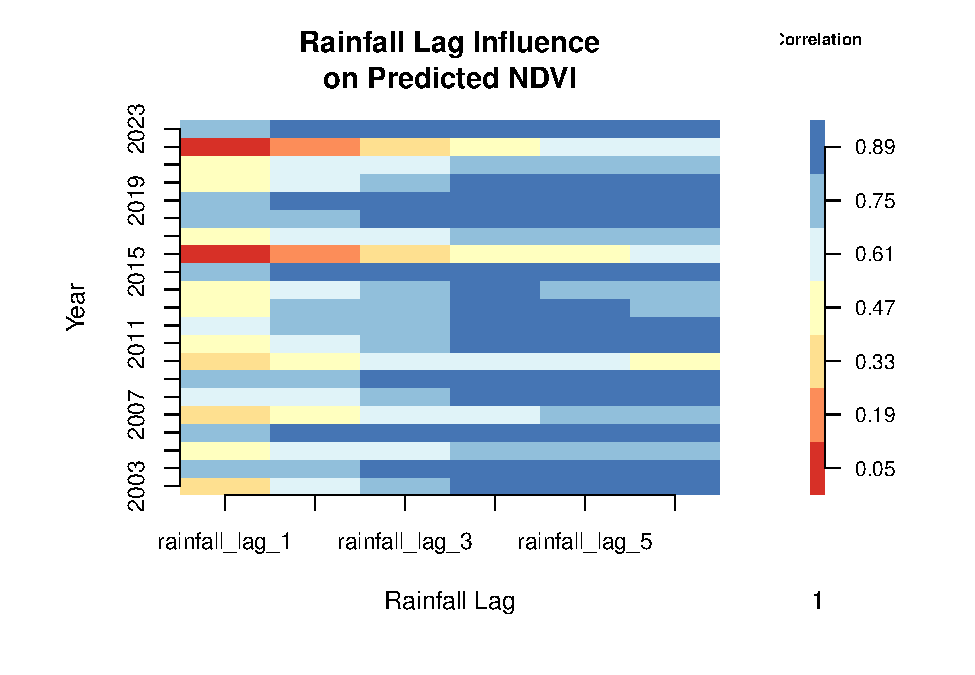
\includegraphics{BI_VegetationResponse_Project_HarvardX_Ph125_9x_files/figure-latex/vis_rainfall_influence_heatmap-1} \end{center}

The \textbf{Rainfall Lag Influence Heatmap} illustrates the correlation
between lagged rainfall variables and predicted NDVI values across
years. The color scale is based on the RdYlBu palette, where:

\begin{itemize}
\tightlist
\item
  Red areas indicate a \textbf{positive correlation} between rainfall
  lag and NDVI, meaning that higher rainfall in that lag period tends to
  result in higher predicted NDVI values.
\item
  Blue areas indicate a \textbf{negative correlation}, suggesting that
  higher rainfall in that lag period is associated with lower predicted
  NDVI values.
\end{itemize}

This heatmap helps to uncover how different time lags of rainfall
influence vegetation health, as captured by the Random Forest model. By
showing correlations for each year, we can identify patterns in how
rainfall impacts vegetation, with certain lags having more influence in
specific years. The analysis is crucial for understanding the temporal
relationships between rainfall and NDVI and for improving the prediction
of vegetation health in response to rainfall variability.

These visualizations complement the model performance metrics by
providing a deeper understanding of how well the \textbf{Random Forest}
model captures seasonal and lagged responses in NDVI based on rainfall.
This can further aid in \textbf{environmental monitoring} and
\textbf{agricultural planning} in regions like \textbf{Indramayu}, where
understanding rainfall's influence on vegetation health is critical for
\textbf{decision-making}.

\begin{center}\rule{0.5\linewidth}{0.5pt}\end{center}

\section{Conclusion and Future Work}\label{conclusion-and-future-work}

\subsection{Summary of Findings}\label{summary-of-findings}

In this study, we successfully developed and tested three predictive
models--- \textbf{Random Forest}, \textbf{Linear Regression}, and
\textbf{ARIMAX}---to estimate NDVI values using rainfall data for the
\textbf{Indramayu} region. Through a comparative analysis of the models,
the \textbf{Random Forest} model emerged as the most effective, offering
the lowest \textbf{RMSE} and \textbf{MAE} values, suggesting it was
better at capturing non-linear relationships and the lagged response of
vegetation to rainfall.

The \textbf{NDVI Difference Heatmap} provided a visual representation of
the NDVI prediction errors across time (years and dekads), showing
periods where the model over- or under-predicted NDVI values.
Additionally, the \textbf{Rainfall Lag Influence Heatmap} revealed that
the \textbf{rainfall lags} were significant in influencing NDVI
predictions, confirming the time-delayed effect of rainfall on
vegetation health. Together, these visualizations complemented the
quantitative performance metrics, providing insights into the models'
effectiveness in predicting NDVI based on rainfall patterns.

\subsection{Limitations}\label{limitations}

While the \textbf{Random Forest} model outperformed the \textbf{Linear
Regression} and \textbf{ARIMAX} models, several challenges were
encountered:

\begin{enumerate}
\def\labelenumi{\arabic{enumi}.}
\item
  \textbf{Data Noise and Temporal Dependencies}: Environmental datasets
  often include a high degree of noise and inherent variability. Factors
  such as cloud cover, soil moisture, and other climatic influences were
  not explicitly captured in the model, potentially affecting the
  accuracy of predictions.
\item
  \textbf{Temporal Scale}: Although we accounted for lagged rainfall
  effects, capturing the full complexity of temporal dependencies---such
  as multi-year drought cycles---remains difficult. The model was
  limited by the temporal granularity of the dekadal NDVI and rainfall
  data.
\item
  \textbf{Model Assumptions}: The \textbf{Random Forest} model, while
  effective at capturing non-linear interactions, may not account for
  complex interactions between rainfall, temperature, and other
  environmental variables. Additionally, the ARIMAX model requires
  stationary time series data, which may not fully represent the complex
  dynamics of vegetation growth.
\item
  \textbf{Dataset Constraints}: The available data from \textbf{2003 to
  2023} constrained the model's ability to capture longer-term trends or
  more recent events that could have impacted vegetation health.
  Furthermore, the \textbf{spatial resolution} of the NDVI and rainfall
  data might limit its application in areas with complex microclimates.
\end{enumerate}

\subsection{Future Work}\label{future-work}

There are several avenues for improving this study and expanding its
applicability:

\begin{enumerate}
\def\labelenumi{\arabic{enumi}.}
\item
  \textbf{Incorporation of Satellite Data for Spatial Resolution}:
  Future studies could integrate higher-resolution satellite data (e.g.,
  Sentinel-2 or Landsat) to improve spatial granularity. This would
  allow for a finer-scale understanding of NDVI variations and more
  precise modeling of localized vegetation health.
\item
  \textbf{Inclusion of Additional Variables}: Incorporating other
  environmental variables, such as soil moisture, temperature, or
  evapotranspiration, could help capture the full range of influences on
  NDVI. Additionally, exploring the impact of extreme weather events
  (e.g., droughts or floods) could improve the robustness of the model.
\item
  \textbf{Temporal Expansion}: Extending the time frame of the study to
  capture more historical or future data could reveal trends and
  cyclical patterns in vegetation health that are currently
  underrepresented in this dataset.
\item
  \textbf{Machine Learning Innovations}: Future work could explore
  advanced machine learning models, such as \textbf{neural networks}
  (e.g., \textbf{LSTM}) or \textbf{hybrid approaches} combining multiple
  models to capture both short-term and long-term dependencies in the
  NDVI-rainfall relationship.
\item
  \textbf{Application in Other Regions}: The approach demonstrated here
  could be applied to other regions with different climate patterns,
  allowing for a comparative analysis of NDVI responses to rainfall
  globally. This would help assess the generalizability of the model
  across various ecosystems.
\end{enumerate}

Overall, while this study has provided valuable insights into the
relationship between rainfall and NDVI, future improvements in data
integration, model sophistication, and geographic coverage will further
enhance the accuracy and applicability of these predictive models for
environmental monitoring and agricultural planning.

\begin{center}\rule{0.5\linewidth}{0.5pt}\end{center}

\section{References}\label{references}

\begin{itemize}
\tightlist
\item
  \textbf{Dataset References}:

  \begin{itemize}
  \tightlist
  \item
    Funk, C., Peterson, P., Landsfeld, M. et al.~The climate hazards
    infrared precipitation with stations---a new environmental record
    for monitoring extremes. Sci Data 2, 150066 (2015).
    \url{https://doi.org/10.1038/sdata.2015.66}
  \item
    Didan, K. (2021). MODIS/Terra Vegetation Indices 16-Day L3 Global
    0.05Deg CMG V061 {[}Data set{]}. NASA EOSDIS Land Processes
    Distributed Active Archive Center. Accessed 2024-09-26 from
    \url{https://doi.org/10.5067/MODIS/MOD13C1.061}
  \item
    Didan, K. (2021). MODIS/Aqua Vegetation Indices 16-Day L3 Global
    0.05Deg CMG V061 {[}Data set{]}. NASA EOSDIS Land Processes
    Distributed Active Archive Center. Accessed 2024-09-26 from
    \url{https://doi.org/10.5067/MODIS/MYD13C1.061}
  \end{itemize}
\item
  \textbf{Software and Libraries}:

  \begin{itemize}
  \tightlist
  \item
    R Core Team. (2021). ``R: A Language and Environment for Statistical
    Computing.''
  \item
    Liaw, A., \& Wiener, M. (2002). ``Classification and Regression by
    randomForest.'' R News, 2(3), 18-22.
  \item
    Hyndman, R. J., \& Khandakar, Y. (2008). ``Automatic Time Series
    Forecasting: The forecast Package for R.'' Journal of Statistical
    Software, 27(3), 1-22.
  \end{itemize}
\item
  \textbf{Environmental Modeling}:

  \begin{itemize}
  \tightlist
  \item
    Chuvieco, E., \& Huete, A. (2010). ``Fundamentals of Satellite
    Remote Sensing.'' CRC Press.
  \item
    Tucker, C. J. (1979). ``Red and Photographic Infrared Linear
    Combinations for Monitoring Vegetation.'' Remote Sensing of
    Environment, 8, 127-150.
  \end{itemize}
\item
  \textbf{Machine Learning for Environmental Applications}:

  \begin{itemize}
  \tightlist
  \item
    Breiman, L. (2001). ``Random Forests.'' Machine Learning, 45, 5--32.
  \item
    James, G., Witten, D., Hastie, T., \& Tibshirani, R. (2013). ``An
    Introduction to Statistical Learning with Applications in R.''
    Springer.
  \end{itemize}
\end{itemize}

\end{document}
